\documentclass[11pt,a4paper]{article}

\usepackage[T1]{fontenc}
\usepackage[utf8]{inputenc}
\usepackage{lmodern}
\usepackage[margin=1in]{geometry}
\usepackage{microtype}
\usepackage{amsmath,amssymb,amsthm}
\usepackage{booktabs}
\usepackage{longtable}
\usepackage{array}
\usepackage{tabularx}
\usepackage{graphicx}
\usepackage{xcolor}
\usepackage{listings}
\usepackage{algorithm}
\usepackage{algorithmic}
\usepackage{tikz}
\usetikzlibrary{arrows.meta,positioning,fit,calc,shapes.geometric,matrix}
\usepackage{enumitem}
\usepackage{titlesec}
\usepackage{fancyhdr}
\usepackage{caption}
\usepackage[numbers,sort&compress]{natbib}
\usepackage{url}
\usepackage[hidelinks]{hyperref}

\definecolor{sirusblue}{RGB}{20,52,96}
\definecolor{sirusgray}{RGB}{92,98,108}
\hypersetup{
  colorlinks=true,
  linkcolor=sirusblue,
  citecolor=sirusblue,
  urlcolor=sirusblue,
  pdftitle={Sirus: A Zero-Dependency, Safe-Rust Code Virtualizer for Selective x86-64 Protection},
  pdfauthor={The Sirus Project},
  pdfsubject={Software protection, code virtualization, obfuscation, constant-time execution},
  pdfkeywords={code virtualization, software obfuscation, mixed Boolean-arithmetic, safe Rust, constant-time, binary rewriting}
}

\titleformat{\section}{\Large\bfseries\color{sirusblue}}{\thesection}{0.8em}{}
\titleformat{\subsection}{\large\bfseries\color{sirusblue}}{\thesubsection}{0.7em}{}
\titleformat{\subsubsection}{\normalsize\bfseries}{\thesubsubsection}{0.6em}{}
\setlength{\parindent}{0.25in}
\setlength{\parskip}{0.15em}
\setlength{\emergencystretch}{3em}
\setlist[itemize]{topsep=0.25em,itemsep=0.1em,parsep=0.1em}
\setlist[enumerate]{topsep=0.25em,itemsep=0.1em,parsep=0.1em}
\captionsetup{font=small,labelfont=bf}
\renewcommand{\arraystretch}{1.08}

\pagestyle{fancy}
\fancyhf{}
\fancyhead[L]{\small\color{sirusgray}Sirus Technical White Paper}
\fancyhead[R]{\small\color{sirusgray}Version 1.5.9-hardened}
\fancyfoot[C]{\small\thepage}
\renewcommand{\headrulewidth}{0.4pt}

\newcommand{\sys}{\textsc{Sirus}}
\newcommand{\code}[1]{\texttt{\detokenize{#1}}}
\newcommand{\etal}{\textit{et al.}}
\newcommand{\eg}{e.g.,}
\newcommand{\ie}{i.e.,}

\newtheorem{definition}{Definition}
\newtheorem{proposition}{Proposition}
\newtheorem{remark}{Remark}

\begin{document}

\begin{titlepage}
\centering
\vspace*{1.2in}
{\color{sirusblue}\rule{\textwidth}{1.2pt}}\\[0.5em]
{\Huge\bfseries Sirus\par}
\vspace{0.35em}
{\LARGE A Zero-Dependency, Safe-Rust Code Virtualizer\\[0.2em]
for Selective x86-64 Protection\par}
\vspace{0.5em}
{\color{sirusblue}\rule{\textwidth}{1.2pt}}\\[1.5em]
{\large Technical White Paper\par}
\vspace{1.2em}
{\large The Sirus Project\par}
\vspace{0.4em}
{\large Version 1.5.9-hardened\par}
\vspace{0.4em}
{\large November 2026\par}
\vfill
\begin{minipage}{0.82\textwidth}
\small
\textbf{Artifact.} The implementation, verification harnesses, recorded results, and
release scripts are maintained at
\url{https://github.com/FutureProofsTech/Sirus}. The paper describes the
\code{1.5.9-hardened} release tree. All quantitative results are taken from
executions recorded in the repository or from the public Windows CI run for the
release; no result is inferred from a vendor claim or from an unexecuted tool.
\end{minipage}
\vspace{1.0em}

{\small Licensed under GPL-3.0-only.}
\end{titlepage}

\begin{abstract}
\noindent
Selective code virtualization protects small, security-sensitive functions by
replacing their native instruction streams with an encrypted virtual instruction
set executed by an interpreter. This paper presents \sys{}, a complete
binary-level virtualizer for Linux ELF64 and Windows PE32+ that is implemented
almost entirely in safe Rust and ships without third-party runtime crates. The
build pipeline lifts a selected x86-64 function into a bounded typed IR, flattens
its control flow, rewrites arithmetic through exact mixed Boolean-arithmetic
identities, encodes the result into a per-build randomized ISA with four aliases
per semantic operation, encrypts the resulting manifest and block bodies, and
synthesizes a freestanding \code{no_std} VM that is injected into a new
read-execute segment. The original function body is overwritten and the entry
point is redirected to an ABI-preserving thunk.

We describe the design in full: the strict x86-64 subset and its fail-closed
decoder, the register and flag model, the bounded IR and CFG flattening, the
linear and non-linear MBA layer, the randomized wire format, the rolling-key body
stream, the SipHash-based integrity binding, the masked at-rest state, the
constant-time oblivious execution mode, and the optional unsafe hardening tier.
We then evaluate the artifact with differential execution, 226 tests, Kani,
Miri, libFuzzer, Ghidra, radare2, angr, KLEE, Creusot, GAMBA, SiMBA, MBA-Blast,
dudect-bencher, Cachegrind, Wine, native Windows, and MSVC \code{/guard:cf}.
The measured results show that the protected function preserves native behavior
across the supported subset, that the generated runtime is memory-safe under the
tested models, that the constant-time subset is below the conventional
\code{|t| = 5} timing threshold on the recorded runs, and that the default
branchy profile remains a measurable timing leak. Coverage is 87.07\% by
tarpaulin and 88.25\% of lines by llvm-cov.

The paper is explicit about what the system does not prove. \sys{} is an
asymmetric-cost engineering prototype, not an indistinguishability obfuscator:
it does not support external calls, host pointers, writable RIP-relative globals,
indirect jumps, floating point, or the full x86-64 ISA, and it does not provide
kernel anti-debug, trusted signing, a formal Spectre proof, or a proof of
obfuscation security. We document those boundaries, the measured residual
equality between builds, the assumptions behind the integrity binding, and the
threats to validity of the evaluation.
\end{abstract}

\vspace{0.5em}
\noindent\textbf{Keywords:} code virtualization, software obfuscation, mixed
Boolean-arithmetic, safe Rust, constant-time execution, binary rewriting,
software protection.

\tableofcontents
\newpage

\section{Introduction}

\subsection{Motivation}

Software often contains small functions whose logic is commercially or
operationally sensitive: license checks, protocol constants, key-derivation
steps, anti-tamper predicates, and proprietary integer algorithms. The defender
cannot generally prevent a determined local attacker from observing a program:
the attacker has the binary, the CPU, the operating system, and arbitrary
instrumentation. What the defender can do is raise the cost of recovering the
function's logic and make a recovered artifact specific to one build.

Code virtualization is one of the strongest practical transformations available
for this problem. Instead of protecting a native instruction stream in place, the
protector translates the selected function into a private instruction set and
executes that instruction set with an embedded interpreter. The original
instructions disappear from the image, the bytecode can be encrypted and
shuffled, and the interpreter can be diversified per build. The cost is a
substantial runtime overhead and a strict limit on the code that can be lifted.

Commercial virtualizers such as VMProtect, Code Virtualizer, Themida, and
Denuvo are mature, closed products with full instruction-set coverage, packing,
anti-debug, licensing, and multi-platform support. Research systems such as
Tigress, Obfuscator-LLVM, and MOVfuscator explore complementary points in the
design space. Sirus occupies a deliberately narrower point: a reproducible,
source-auditable, zero-dependency implementation for selected x86-64 leaf
functions, built in safe Rust, with a measured evidence trail rather than
vendor claims.

\subsection{Problem statement}

Given an ELF64 or PE32+ AMD64 image $B$ and a selected function $f$ that belongs
to a supported x86-64 subset, Sirus must produce an image $B'$ such that:

\begin{enumerate}
  \item $B'$ preserves the observable integer behavior of $f$ on supported
        inputs and the supported ABI;
  \item the original bytes of $f$ no longer contain a readable native
        implementation;
  \item the replacement is not a single fixed interpreter shared by all builds,
        but a per-build randomized artifact whose opcode assignment, operand
        layout, register encoding, state identifiers, payload encryption, and
        code/data placement depend on a 256-bit seed;
  \item the generated runtime is memory-safe under the Rust type system, uses
        no heap, no libc, and no host memory, and fails closed on malformed
        bytecode;
  \item the result can be reproduced exactly from the input, seed, profile, and
        pinned toolchain, and the evidence for each security and correctness
        claim can be re-executed locally.
\end{enumerate}

The problem is deliberately not "construct an indistinguishability obfuscator."
Barak \etal{} showed that general-purpose obfuscation with strong
virtual-black-box properties is impossible for arbitrary programs
\cite{barak2012}. Practical protectors therefore aim at cost asymmetry,
build-specific diversity, and resistance to specific automated analyses. Sirus
follows that realistic objective.

\subsection{Contributions}

This paper makes the following contributions.

\begin{enumerate}
  \item \textbf{A complete selective virtualizer.} We describe and evaluate an
        end-to-end pipeline that parses and edits ELF64 and PE32+ images, lifts a
        strict x86-64 subset into a bounded IR, flattens control flow, rewrites
        arithmetic, encodes a randomized ISA, synthesizes a freestanding
        \code{no_std} Rust VM, injects it into a new read-execute segment, and
        scrubs the original body.

  \item \textbf{A randomized encrypted ISA.} The virtual instruction set has 48
        semantic operations and four aliases per operation. Each alias has its
        own operand order, one of two register encoding maps, and an immediate
        endianness bit. The runtime decode table is itself encrypted and derived
        from the build seed; the alias layout is not serialized as plaintext in
        the executable.

  \item \textbf{A layered obfuscation stack.} The pipeline combines CFG
        flattening with random state identifiers, opaque guards, decoy blocks,
        bounded linear MBA, a non-linear modular-inverse wrapper, constant
        blinding, a rolling-key ARX body stream, SipHash-based integrity and key
        binding, and masked virtual registers and private memory at rest.

  \item \textbf{A fixed-pass oblivious execution mode.} The optional
        \verb|--constant-time| path executes every manifest block on every pass,
        carries the active path in frontier masks, predicates register writes,
        enqueues both branch successors with complementary masks, and scans the
        whole private stack for loads and stores. We state the exact property it
        provides, the pass bound it assumes, and the microarchitectural effects it
        does not model.

  \item \textbf{An evidence-driven evaluation.} We report 226 tests in debug and
        release modes, Kani and Miri results, more than 40 million recorded
        libFuzzer executions across VM, lifter, ELF, and PE targets, differential
        execution against native code, tamper and forced-return experiments,
        Ghidra and radare2 decompilation, bounded angr and KLEE probes, Creusot
        boundary proofs, three external MBA simplifiers, dudect-bencher,
        Cachegrind, Wine, native Windows, and an MSVC \code{/guard:cf} fixture.
        We also report the negative results: the default branchy profile leaks
        timing, GAMBA and SiMBA reduce parts of the MBA layer, one Ghidra
        decompilation exceeds its budget, and the symbolic probes time out rather
        than prove unsatisfiability.

  \item \textbf{A documented boundary.} We enumerate the supported instruction
        subset, ABI limits, platform limits, unsupported attacks, and the
        assumptions behind the integrity binding. The paper does not claim
        kernel-level anti-debug, trusted signing, a formal Spectre proof, or a
        proof of obfuscation security.
\end{enumerate}

\subsection{Artifact and reproducibility}

The artifact is a Cargo workspace with four shipped crates
(\code{sirus-core}, \code{sirus-vm}, \code{sirus-binfmt},
\code{sirus-protector}), an excluded fuzzing crate, and external verification
harnesses under \path{verification/} and \path{scripts/}. The release is
\code{1.5.9-hardened}. The fast gate is \path{scripts/verify.sh}; the long proof
and fuzzing gate is \path{scripts/prove.sh}. The public Windows CI workflow
executes Wine, native Windows, and MSVC \code{/guard:cf} jobs.

A fixed input, seed, profile, and toolchain produce a bit-identical protected
image. The differential test harness compiles the same C source twice, protects
selected functions with a fixed seed, and compares native and protected results
over thousands of random inputs. The measurement scripts and their outputs are
part of the repository, so a reader can distinguish a reproduced result from a
quoted one.

\subsection{Non-goals}

Sirus is not a whole-program virtualizer, a packer, a licensing system, or a
replacement for a formally audited protector. It does not support external
calls, indirect calls or jumps, writable RIP-relative globals, host pointers,
floating point, x87, AVX-256, other instruction-set extensions, syscalls,
atomics, or arbitrary platform ABIs. It does not implement kernel anti-debug or
guarantee security against an attacker with unlimited local instrumentation. The
default profile is not constant-time. These are design boundaries, not hidden
failure modes: unsupported inputs fail the build, and unsupported runtime states
fail closed with a deterministic status.

\subsection{Organization}

Section~\ref{sec:threat} defines the adversary and objectives.
Section~\ref{sec:background} reviews obfuscation, virtualization, MBA, binary
analysis, and timing measurement. Section~\ref{sec:overview} gives the system
overview. Sections~\ref{sec:frontends}--\ref{sec:runtime} describe the binary
front ends, lifting, obfuscation, and VM runtime.
Section~\ref{sec:constant-time} presents the oblivious mode;
Section~\ref{sec:hardening} describes the optional hardening tier;
Section~\ref{sec:implementation} covers safety engineering.
Section~\ref{sec:evaluation} reports the evaluation, and
Sections~\ref{sec:security}--\ref{sec:conclusion} analyze residual risk and
conclude. The appendices contain the full virtual ISA, the x86-64 subset, the
verification matrix, reproduction commands, and a glossary.

\section{Threat Model and Security Objectives}
\label{sec:threat}

\subsection{Assets}

Sirus is intended to protect four classes of assets:

\begin{itemize}
  \item \textbf{Proprietary integer logic}: license predicates, protocol
        constants, checksums, and business rules.
  \item \textbf{Embedded secrets}: salts, derivation keys, and constants that
        participate in a larger key schedule.
  \item \textbf{Algorithm structure}: the control flow and arithmetic shape that
        reveal how a decision is made.
  \item \textbf{Build geometry}: the per-build ISA assignment, register maps,
        decode-table key, and payload keys that make one protected image
        different from another.
\end{itemize}

The protected function is assumed to be a leaf or a small cluster of directly
called functions. Its result is consumed by the host as data, not as a single
boolean that an attacker can patch at the call site without consequence.

\subsection{Adversary capabilities}

We assume an adversary who can:

\begin{itemize}
  \item read the complete binary, symbol table, section headers, and metadata;
  \item run disassemblers and decompilers, including Ghidra, IDA, Binary Ninja,
        radare2, and custom parsers;
  \item run MBA simplifiers such as GAMBA, SiMBA, and MBA-Blast;
  \item run symbolic execution and SMT solvers such as angr, KLEE, Triton, and
        Z3;
  \item trace execution with Intel PIN, Frida, DynamoRIO, QEMU, gdb, or a
        hypervisor;
  \item dump process memory at any time, including during an executing
        instruction;
  \item patch file or memory bytes, including the generated entry thunk;
  \item compare two protected builds of the same source;
  \item fuzz the VM with malformed, truncated, or mutated payloads;
  \item use hardware breakpoints and debug registers.
\end{itemize}

The adversary is \emph{not} assumed to have unlimited CPU time in the intended
cost model. Sirus is an asymmetry mechanism: the defender pays a bounded
compile-time and runtime cost, and the attacker is forced through a larger
search, decoding, and analysis space. An adversary with unlimited time and full
instrumentation can eventually recover behavior; no claim in this paper
contradicts that.

\subsection{Security objectives}

Table~\ref{tab:objectives} states the objectives and the controls that address
them. The evidence column identifies the class of evidence, not a proof of
absolute security.

\begin{table}[htbp]
\centering
\small
\caption{Security objectives and current controls.}
\label{tab:objectives}
\begin{tabularx}{\textwidth}{@{}>{\raggedright\arraybackslash}p{0.06\textwidth}>{\raggedright\arraybackslash}p{0.25\textwidth}>{\raggedright\arraybackslash}p{0.35\textwidth}>{\raggedright\arraybackslash}X@{}}
\toprule
ID & Objective & Control & Evidence \\
\midrule
O1 & Remove readable original logic & Original body scrubbed; bytecode flattened, shuffled, and encrypted & Patch/scrub checks; Ghidra and radare2 output \\
O2 & Obscure operations & Bounded linear and non-linear MBA; constant blinding; randomized ISA & MBA equivalence tests; external simplifier study \\
O3 & Make builds independent & New seed changes opcodes, operand order, register maps, state ids, block order, keys, MBA shapes, decoys, and layout & Differential payload and segment equality \\
O4 & Detect payload tampering & SipHash-derived integrity value mixed into the effective payload key & Tamper experiments produce deterministic wrong output \\
O5 & Keep the host safe & Safe Rust, checked decode, no heap, fuel bound, private memory, fail-closed status & Kani, Miri, libFuzzer, malformed-payload suite, valgrind \\
O6 & Resist forced-return bypass & Protected results are data consumed downstream; wrong values change observable output & Forced-return experiment \\
O7 & Avoid leaked VM strings & Generated engine uses no formatting, panic strings, or libc symbols & Static string scan of the injected segment \\
\bottomrule
\end{tabularx}
\end{table}

\subsection{Non-objectives}

The following are explicitly outside the threat model:

\begin{itemize}
  \item protection against an adversary with unlimited local time and full
        hardware instrumentation;
  \item kernel-level anti-debugging or DBI detection in the safe tier;
  \item hiding the existence of a VM or of the protected entry points;
  \item preventing a caller-side patch that ignores the protected result;
  \item a formal cryptographic proof for the custom payload construction;
  \item whole-program virtualization;
  \item protecting functions that require external calls, host memory, floating
        point, or unsupported instructions;
  \item trusted production signing or an independent audit.
\end{itemize}

\subsection{Failure policy}

The runtime distinguishes five outcomes: \code{Returned}, \code{BadPayload},
\code{FuelExhausted}, \code{Trap}, and \code{LoopBound}. A malformed payload,
an invalid register, an out-of-range memory access, a missing manifest entry, an
invalid opcode, or an exhausted fuel budget never unwinds and never accesses host
memory. It returns value zero with the corresponding status. The build-time
pipeline similarly fails with a typed error and does not write a partial output
file.

Returning zero is not itself a security guarantee. The intended deployment
consumes the protected result as data in a downstream computation, so an
incorrect result causes an observable failure rather than a silent success.

\subsection{Cost model and evidence discipline}

We evaluate the system along three axes: correctness, safety, and recovery cost.
Correctness is measured by differential execution on real binaries. Safety is
measured by the Rust type system, bounded proofs, dynamic analysis, and fuzzing.
Recovery cost is measured by differential builds, external static and symbolic
tools, MBA simplifiers, and timing measurements. Each result is reported with
its scope. A Kani harness that proves a bounded memory helper is not presented as
a proof of the dispatcher; a Ghidra timeout is not presented as a proof that
decompilation is impossible; a dudect run below the threshold is not presented as
a formal constant-time proof.

The following terminology is used throughout:

\begin{definition}[Measured equality]
For two protected images $B'_0$ and $B'_1$ of the same input under different
seeds, the \emph{equal-byte ratio} of a section is the number of byte positions
with identical values at the same relative offset, divided by the section length.
It is a diversity metric, not a semantic security proof.
\end{definition}

\begin{definition}[Bounded symbolic resistance]
A symbolic probe is \emph{bounded-resistant} for a time budget $T$ if it does not
produce a concrete preimage for the requested target within $T$. A timeout is
evidence of cost, not a proof of unsatisfiability.
\end{definition}

\begin{definition}[Fixed-pass oblivious execution]
An execution is \emph{fixed-pass oblivious} with respect to a set of secret
inputs if, for a fixed program and pass bound $P$, the sequence of decoded basic
blocks and the sequence of private-memory addresses are independent of those
inputs, provided the active frontier converges within $P$. Register values and
branch conditions may still depend on the inputs.
\end{definition}

\section{Background and Related Work}
\label{sec:background}

\subsection{Obfuscation and virtualization}

Software obfuscation is the systematic transformation of a program to make its
behavior harder to recover while preserving semantics. Collberg, Thomborson, and
Low classified transformations into layout, data, control, and preventive
families \cite{collberg1997,collberg2002}. Control-flow flattening replaces a
structured CFG with a dispatcher over state variables; data transformations
rewrite expressions and constants; preventive transformations detect or impede
debuggers and analysis tools. Banescu and Pretschner give a modern tutorial and
taxonomy \cite{banescu2018}.

Code virtualization is a control transformation in which the protected function
is translated into a bytecode program for a private interpreter. The interpreter
and bytecode are embedded in the binary. The original native instructions can be
removed, and the bytecode can be encrypted, shuffled, and diversified. The
approach is attractive because it changes the attacker's problem from reading
native instructions to recovering both the ISA and the program. It is expensive
because every virtual instruction requires dispatch, decode, and interpretation.

Barak \etal{} proved that general-purpose obfuscation with strong
virtual-black-box security is impossible for arbitrary programs
\cite{barak2012}. The result does not rule out practical protection: it rules out
a universal transformation that hides all properties of every program. Sirus
therefore targets cost asymmetry and build-specific diversity, not
indistinguishability.

\subsection{Commercial protectors}

VMProtect is a commercial protector with virtualization, mutation, packing,
anti-debug, and licensing features \cite{vmprotect}. Code Virtualizer and Themida
from Oreans provide selective virtualization, multiple VM architectures, packing,
and anti-debug controls \cite{codevirtualizer,themida}. Denuvo Anti-Tamper is a
game-oriented product with its own virtual machine and integrity checks
\cite{denuvo}. These products are mature and support much broader instruction
sets and platforms than Sirus. Their internals are not public, and their security
claims are vendor-documented rather than independently reproduced in this work.

The comparison in this paper is deliberately narrow. We use VMProtect 3.11 Linux
demo as a measured performance peer because it can virtualize the same benchmark
function on the same host. We do not claim equivalence of security profiles,
packing, anti-debug, licensing, or platform coverage.

\subsection{Research systems}

Tigress is a source-to-source C transformer with a broad set of diversification
transformations, including virtualization, superoperators, reentrant interpreters,
anti-taint, and anti-aliasing passes \cite{tigress}. It is the closest research
peer in ambition, but it operates at source level and is not a binary protector.
Obfuscator-LLVM implements control-flow flattening, instruction substitution, and
bogus control flow at the LLVM IR level \cite{junod2015ollvm}; it is not a
virtualizer. MOVfuscator compiles programs into `mov'-only code as a research
demonstration \cite{domas2015movfuscator}; its cost profile is intentionally
extreme and it is not a selective production protector.

Sirus differs from these systems in three ways: it operates directly on ELF and
PE binaries, it is implemented in safe Rust with no third-party runtime crates,
and it ships an evidence harness that executes the protected binaries and the
external analysis tools. The trade-off is a strict instruction subset and a
narrow platform scope.

\subsection{Mixed Boolean-arithmetic obfuscation}

Mixed Boolean-arithmetic (MBA) expressions combine bitwise operations with
integer addition, subtraction, and multiplication. Zhou \etal{} showed that such
expressions can hide simple arithmetic and proposed rewrite-based
simplification \cite{zhou2007}. Modern simplifiers exploit the fact that a linear
MBA expression over $n$ variables is determined by its values on the $2^n$
Boolean inputs, and use linear algebra over the bit-vector space to recover a
compact form. GAMBA generalizes the approach to selected non-linear expressions
\cite{reichenwallner2023gamba}; SiMBA specializes in linear expressions
\cite{reichenwallner2022simba}; MBA-Blast is another widely used
simplifier \cite{mba_blast}.

Sirus uses a layered approach. Exact linear identities provide a baseline
rewrite, and one non-linear wrapper per function adds variable shifts and a
data-dependent modular inverse. The external simplifier study in
Section~\ref{sec:evaluation} reports both the reductions and the failures. The
result is measured cost asymmetry, not a claim that the expressions are
irreducible.

\subsection{Binary analysis and symbolic execution}

Ghidra \cite{ghidra} and radare2 \cite{radare2} are open reverse-engineering
frameworks used for static decompilation and disassembly. angr is a Python
binary-analysis platform with symbolic execution, constraint solving, and data
flow analysis \cite{shoshitaishvili2016angr}. KLEE is a symbolic execution engine
for LLVM bitcode that generates high-coverage test inputs and checks memory
safety \cite{cadar2008klee}. Z3 is the SMT solver commonly used by these tools
\cite{z3_2008}. PIN and DynamoRIO are dynamic instrumentation frameworks that can
trace a running process at instruction granularity \cite{pin2005}.

Sirus does not attempt to defeat these tools in the sense of a formal
impossibility result. It increases the size of the state space through encrypted
bytecode, randomized state identifiers, flattened control flow, MBA, and a
bounded fuel budget. The evaluation records what the tools did within fixed
budgets and treats a timeout as bounded resistance.

\subsection{Constant-time execution and timing measurement}

Timing attacks exploit data-dependent execution time, memory access patterns, or
microarchitectural state \cite{kocher1996,bernstein2005}. Spectre-class attacks
exploit speculative execution and are not solved by branchless source code
alone \cite{kocher2019spectre}. Constant-time programming therefore targets a
specific class of leakage: the sequence of instructions and memory addresses,
not every microarchitectural effect.

dudect-bencher is a statistical tool that measures whether two input classes are
distinguishable by execution time \cite{reparaz2017dudect}. Cachegrind, part of
Valgrind, provides deterministic instruction and cache-access counts
\cite{nethercote2007valgrind}. Sirus uses both: dudect for wall-clock
distinguishability and Cachegrind for input-independent instruction and address
counts on a controlled leaf function.

\subsection{Rust safety and verification}

Rust's ownership and borrowing rules provide memory and thread safety without a
garbage collector; RustBelt gives a formal foundation for the safe
fragment \cite{jung2018rustbelt,rustref}. Sirus additionally enforces
\code{forbid(unsafe_code)} in the safe tier, forbids heap allocation in the core
and VM, and uses fixed-capacity data structures. Kani provides bounded model
checking for Rust \cite{kani}, Miri detects undefined behavior in the Rust
abstract machine \cite{miri}, and Creusot/Why3 supports deductive verification of
Rust functions \cite{creusot2022,why3_2013}. These tools cover different scopes;
the evaluation states each scope explicitly.

\subsection{Positioning}

Table~\ref{tab:related} summarizes the qualitative position. Commercial entries
are based on public vendor documentation and are marked accordingly; they are not
independently verified in this work.

\begin{table}[htbp]
\centering
\small
\caption{Qualitative positioning. ``Y'' denotes documented or implemented,
``P'' partial or subset, and ``N'' not supported. Commercial entries are
vendor-documented capabilities, not independent measurements.}
\label{tab:related}
\begin{tabularx}{\textwidth}{@{}lcccccc@{}}
\toprule
Capability & Sirus & VMProtect & Code Virtualizer & Themida & Tigress & OLLVM \\
\midrule
Selective virtualization & Y & Y & Y & Y & Y & N \\
Full x86-64 ISA & N & Y & Y & Y & via C & via IR \\
Linux ELF runtime & Y & Y & Y & N & via C & Y \\
Windows PE runtime & P & Y & Y & Y & via C & via C \\
Multiple VM designs & N & Y & Y & Y & Y & N \\
Packing & N & Y & N & Y & N & N \\
Anti-debug / anti-VM & P & Y & P & Y & research & N \\
Runtime integrity & P & Y & P & Y & research & P \\
Safe Rust runtime & Y & N & N & N & N & N \\
Zero runtime crates & Y & N & N & N & N & N \\
Source available & Y & N & N & N & limited & Y \\
Local evidence harness & Y & N/A & N/A & N/A & papers & public \\
\bottomrule
\end{tabularx}
\end{table}

Sirus is best described as a reproducible, selective Linux-first virtualizer
with a Windows leaf-function line, within roughly one order of magnitude of a
commercial per-call VM on the same benchmark, but without the platform coverage,
anti-debug, packing, licensing, or maturity of commercial products. It is not a
replacement for a commercial protector on arbitrary Windows software.

\section{System Overview}
\label{sec:overview}

\subsection{Design principles}

The implementation follows six principles.

\begin{description}[leftmargin=1.4em,style=nextline]
  \item[Fail closed.] The decoder accepts only the documented subset. A branch
        target outside the function, an overlapping instruction, an unknown flag
        producer, an unsupported prefix, or a malformed encoding is a build
        error. The runtime rejects malformed payloads, invalid registers,
        out-of-range memory, invalid opcodes, and exhausted fuel with a
        deterministic status. There is no best-effort translation.
  \item[Zero shipped dependencies.] The compiler core, VM, and binary-format
        layer depend only on \code{core}. The protector CLI uses \code{std} at
        the filesystem, process, and error-reporting boundary. No third-party
        crate is linked into a protected artifact.
  \item[Memory safety by construction.] The safe tier uses
        \texttt{\#![forbid(unsafe\_code)]}. The VM has no heap allocation, no
        unchecked indexing in its public path, no division, no floating point,
        and no host-memory access. Bounds are checked at every decode and memory
        operation.
  \item[Per-build diversity.] A 256-bit seed drives opcode assignment, alias
        operand order, register-map selection, immediate endianness, manifest
        endianness, state identifiers, block order, rolling keys, entry shares,
        MBA shape, decoy placement, semantic-handler order, and code/data
        offsets. Two builds of the same input differ in every payload byte and
        in most of the VM segment.
  \item[Separated unsafe boundary.] Debugger detection, RDTSC/LFENCE, and
        native text checksums require OS interfaces or instructions that safe
        Rust cannot express. They are isolated in an opt-in
        \code{sirus-hardened} crate and generated only with \verb|--hardened|.
  \item[Evidence rather than assertion.] Every security claim is paired with a
        script that can be re-executed. The paper reports negative results and
        tool limitations alongside positive ones.
\end{description}

\subsection{Build pipeline}

Figure~\ref{fig:pipeline} shows the build pipeline. The input image is parsed and
validated; one or more selectors resolve functions; the selected ranges are
decoded and lifted; the resulting CFG is flattened and rewritten; the IR is
encoded into the randomized ISA; the manifest and bodies are encrypted; a
freestanding Rust VM is generated and compiled; the resulting blob is validated;
the blob is injected into a new executable segment; the original entries are
patched; and the original bodies are scrubbed.

\begin{figure}[htbp]
\centering
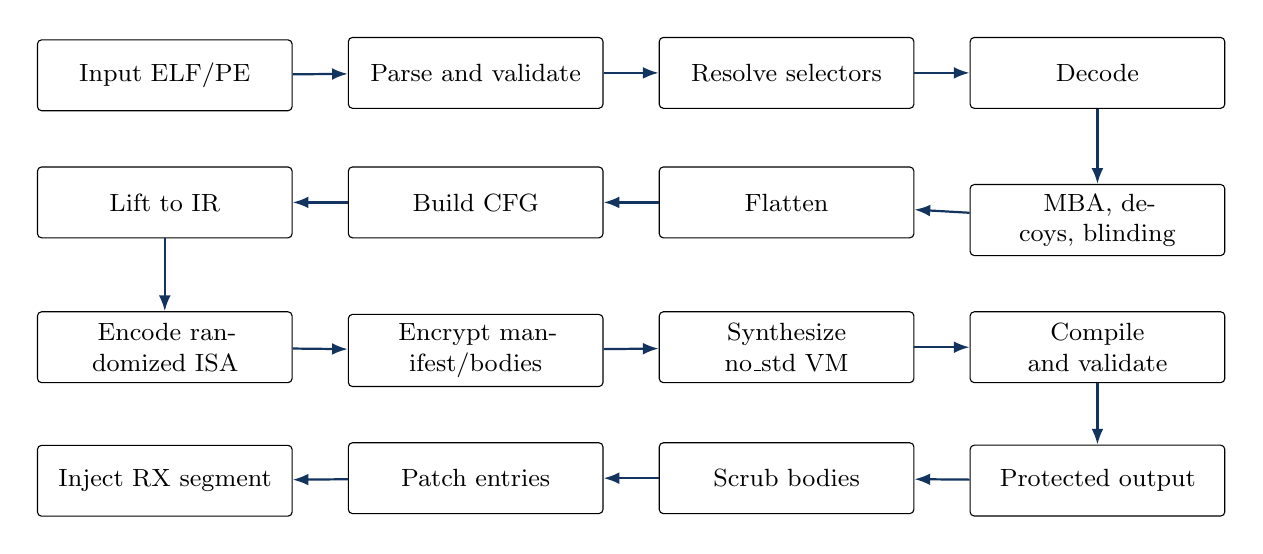
\begin{tikzpicture}[
  box/.style={draw, rounded corners=1.5pt, align=center, text width=30mm,
              minimum height=9mm, font=\small, fill=white},
  arrow/.style={-{Latex[length=2mm]}, thick, color=sirusblue},
  node distance=6mm and 7mm
]
\matrix (m) [matrix of nodes, nodes={box}, row sep=7mm, column sep=7mm] {
  Input ELF/PE & Parse and validate & Resolve selectors & Decode \\
  Lift to IR & Build CFG & Flatten & MBA, decoys, blinding \\
  Encode randomized ISA & Encrypt manifest/bodies & Synthesize no\_std VM & Compile and validate \\
  Inject RX segment & Patch entries & Scrub bodies & Protected output \\
};
\foreach \i [evaluate=\i as \j using int(\i+1)] in {1,2,3} {
  \draw[arrow] (m-1-\i) -- (m-1-\j);
  \draw[arrow] (m-2-\j) -- (m-2-\i);
  \draw[arrow] (m-3-\i) -- (m-3-\j);
  \draw[arrow] (m-4-\j) -- (m-4-\i);
}
\draw[arrow] (m-1-4) -- (m-2-4);
\draw[arrow] (m-2-1) -- (m-3-1);
\draw[arrow] (m-3-4) -- (m-4-4);
\end{tikzpicture}
\caption{Build pipeline. The flow snakes through four rows; each stage is
deterministic for a fixed input, seed, profile, and toolchain.}
\label{fig:pipeline}
\end{figure}

The target binary is never relocated. The ELF program-header table is moved to
an appended read-only page, one new read-only \code{PT_LOAD} maps it, and one
new read-execute \code{PT_LOAD} maps the VM. The original load segments are
untouched. The PE backend appends one read-execute section, updates the section
count and image size, recomputes the checksum, and patches RVA-relative entries.

\subsection{Runtime pipeline}

Figure~\ref{fig:runtime} shows the runtime. A host call reaches a per-function
ABI shim. The shim preserves the host calling convention, materializes register
and stack arguments, and calls the generated entry. The entry derives the
decode tables and payload key from the seed and the integrity value, scans the
encrypted manifest for the entry state, and enters the dispatcher. The dispatcher
decrypts one instruction at a time, resolves the alias, executes the semantic
operation, and transitions to the next state. A return writes the virtual
\code{RAX} value; an error writes zero and a status.

\begin{figure}[htbp]
\centering
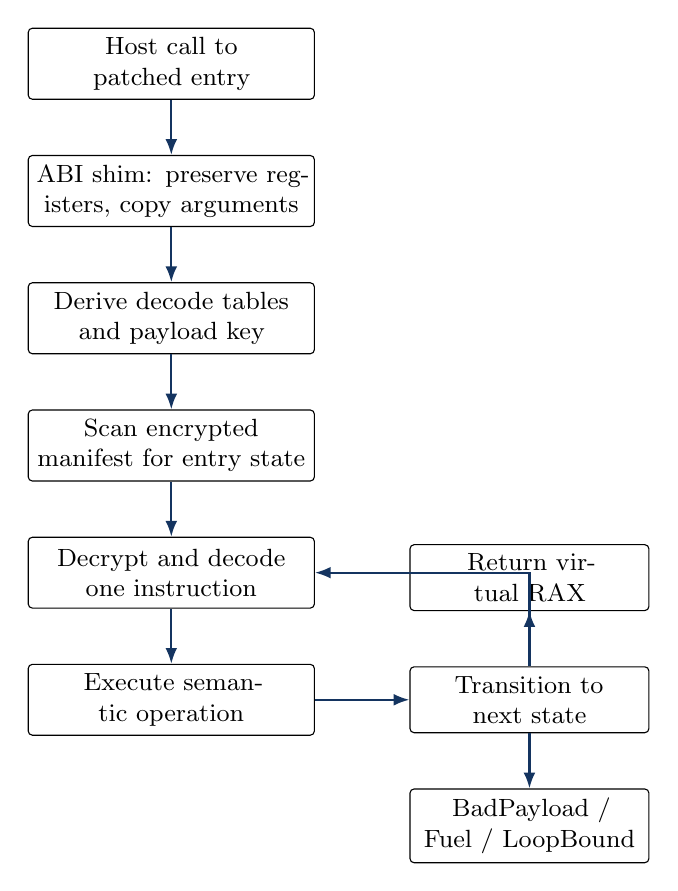
\begin{tikzpicture}[
  box/.style={draw, rounded corners=1.5pt, align=center, text width=34mm,
              minimum height=9mm, font=\small, fill=white},
  smallbox/.style={draw, rounded corners=1.5pt, align=center, text width=28mm,
              minimum height=8mm, font=\small, fill=white},
  arrow/.style={-{Latex[length=2mm]}, thick, color=sirusblue},
  node distance=7mm and 12mm
]
\node[box] (call) {Host call to patched entry};
\node[box, below=of call] (shim) {ABI shim: preserve registers, copy arguments};
\node[box, below=of shim] (init) {Derive decode tables and payload key};
\node[box, below=of init] (manifest) {Scan encrypted manifest for entry state};
\node[box, below=of manifest] (decode) {Decrypt and decode one instruction};
\node[box, below=of decode] (exec) {Execute semantic operation};
\node[smallbox, right=of exec] (next) {Transition to next state};
\node[smallbox, above=of next] (ret) {Return virtual RAX};
\node[smallbox, below=of next] (fail) {BadPayload / Fuel / LoopBound};
\draw[arrow] (call) -- (shim);
\draw[arrow] (shim) -- (init);
\draw[arrow] (init) -- (manifest);
\draw[arrow] (manifest) -- (decode);
\draw[arrow] (decode) -- (exec);
\draw[arrow] (exec) -- (next);
\draw[arrow] (next) |- (decode);
\draw[arrow] (next) -- (ret);
\draw[arrow] (next) -- (fail);
\end{tikzpicture}
\caption{Runtime structure. The transition arrow is the dispatcher loop; the
manifest is scanned once per transition in the normal profile.}
\label{fig:runtime}
\end{figure}

\subsection{Crate architecture and trust boundaries}

The workspace separates concerns by trust level:

\begin{itemize}
  \item \code{sirus-core}: \code{no_std}, no allocation, no unsafe. Decoder,
        lifter, IR, MBA arena, ISA derivation, payload cipher, program builder.
  \item \code{sirus-vm}: \code{no_std}, no allocation, no unsafe. Reference
        engine used by tests and embedded verbatim into generated runtimes.
  \item \code{sirus-binfmt}: \code{no_std} plus \code{alloc}, no unsafe. ELF and
        PE parsers, editors, and injection geometry.
  \item \code{sirus-protector}: \code{std} boundary, safe Rust. Selector
        resolution, source generation, \code{rustc} invocation, blob validation,
        injection, patching, and scrubbing.
  \item \code{sirus-hardened}: opt-in unsafe. Linux and Windows hardening
        primitives; never linked into the safe default runtime.
\end{itemize}

The compiler and runtime share the \code{shared} modules verbatim: the ISA
constants, SipHash, ChaCha20, and decode-table derivation are compiled into both
the protector and the generated VM. This eliminates a class of encoder/decoder
divergence bugs and is checked by the build system, which tracks every embedded
source file and rebuilds the protector when one changes.

The external verification crates (\code{verification/dudect},
\code{verification/creusot}, and \code{fuzz}) are outside the shipped dependency
graph. They may use external crates because they are measurement and proof
tooling, not runtime components.

\subsection{Threat surface}

The protected binary has three relevant surfaces: the host image, the injected
VM segment, and the runtime entry path. The host image retains its symbol table
and dynamic metadata; Sirus does not strip the host. The VM segment contains the
engine, the encrypted payload, the encrypted decode table, and the per-build
constants. The entry path contains the patched jump and the ABI shim. An
attacker can read all three, trace them, and patch them. The design assumes this
and attempts to make the semantic recovery and patch construction expensive, not
impossible.

\section{Binary Front Ends and Injection}
\label{sec:frontends}

\subsection{ELF64 parsing and validation}

The ELF front end accepts 64-bit little-endian x86-64 executables and shared
objects. The parser validates the ELF header, class, data encoding, machine,
program-header table, section-header table, section bounds, load-segment flags,
and the presence of an executable range. Extended numbering (\code{PN_XNUM},
\code{SHN_XINDEX}) and unsupported object types fail closed. Function symbols
are read from \code{.symtab} or \code{.dynsym}; fully stripped inputs require
marker or explicit-range selection.

The editor never relocates the target. It appends new bytes and rewrites the
program-header table in a new read-only page. This avoids moving existing
segments and preserves the host loader's expectations.

\subsection{Selector resolution}

A protection run resolves one or more functions using one of four selectors:

\begin{itemize}
  \item an exact symbol name (\verb|--function|);
  \item a unique symbol substring (\verb|--function-contains|);
  \item an explicit executable RVA and size (\verb|--range|);
  \item raw byte markers (\verb|--marker-begin|/\verb|--marker-end|).
\end{itemize}

The resolved range must lie in an executable segment, must not overlap another
selected range or an already-patched entry, and must decode completely within the
supported subset. Marker mode is intentionally raw: the user is responsible for
placing the markers so that the enclosed bytes form valid machine code.

\subsection{ELF injection geometry}

The appended layout is:

\begin{center}
\small
\begin{tabular}{@{}lll@{}}
\toprule
Region & Mapping & Content \\
\midrule
Original bytes & original segments & unchanged host image \\
Program-header page & \code{R} & relocated \code{PT_PHDR} table \\
VM segment & \code{R+X} & engine, tables, payload, entry thunks \\
\code{.shstrtab} & section metadata & regenerated names \\
Section-header table & section metadata & regenerated entries \\
\bottomrule
\end{tabular}
\end{center}

One new read-only \code{PT_LOAD} maps the relocated program-header table, and one
new read-execute \code{PT_LOAD} maps the VM. The \code{PT_PHDR} entry is updated
to the new table. The section-header table and section-name string table are
regenerated; \code{.sirus} and \code{.sirus.payload} sections are created even
for inputs that lacked a name table.

The injected VM is linked at a chosen virtual address with a custom linker
script. The blob is a single read-execute segment with no writable load, no
relocations, and no undefined symbols. The validator rejects any blob that
violates these properties, any missing entry symbol, any entry outside the
segment, and any payload/seed/hash mismatch.

\subsection{Entry patching and body scrubbing}

The patcher writes \code{E9 <rel32>} at the target entry, or immediately after a
preserved \code{F3 0F 1E FA} (\code{endbr64}) sequence. If the displacement does
not fit in 32 bits, the build fails. The remainder of the original function body
is overwritten with deterministic random bytes derived from the build seed,
unless \verb|--no-scrub| is requested. The output is written to a temporary file
in the destination directory, permissions are copied from the input, and the file
is atomically renamed.

Preserving \code{endbr64} keeps the patched entry a valid indirect-branch target
under Intel CET. The jump itself preserves the host return address: the patched
function is entered by a normal call, and the VM thunk returns normally.

\subsection{PE32+ backend}

The Windows backend accepts PE32+ AMD64 images. It validates the DOS, COFF, and
optional headers, the machine type, section alignment, section bounds, RVA to file
mapping, checksum, and COFF symbol information. Injection appends one
read-execute \code{.sirus} section, updates the section count and
\code{SizeOfImage}, recomputes the PE checksum, patches one RVA-relative jump per
protected function, and overwrites the original body with keyed junk.

The Win64 runtime is cross-compiled with
\code{rustc --target x86_64-pc-windows-gnu}, linked with \code{lld-link}, and
embedded as one section. The generated shim includes a guard-page-safe stack
probe, preserves the Windows calling convention, and translates register and
stack arguments into the VM's internal array. Linked \code{.pdata} entries are
rebased into the section and merged into the target exception directory;
handler-bearing and chained unwind records fail closed.

The tested Windows fixtures cover a normal leaf, constant-time execution, a
hardened self-code checksum, a \code{/guard:cf} binary with indirect callers, a
DLL export loaded through \code{LoadLibrary}/\code{GetProcAddress}, and a TLS
callback plus \code{RCDATA} resource. The native Windows CI job, the Wine job,
and the MSVC \code{/guard:cf} job all pass on the release tree. Signing,
arbitrary imports, runtime exception propagation, and kernel anti-debug remain
out of scope.

\subsection{ABI shims and call semantics}

Table~\ref{tab:abi} summarizes the supported calling conventions.

\begin{table}[htbp]
\centering
\small
\caption{Supported integer ABI surface.}
\label{tab:abi}
\begin{tabularx}{\textwidth}{@{}l>{\raggedright\arraybackslash}X>{\raggedright\arraybackslash}X@{}}
\toprule
Property & System V AMD64 & Win64 \\
\midrule
Register arguments & 6: RDI, RSI, RDX, RCX, R8, R9 & 4: RCX, RDX, R8, R9 \\
Stack arguments & 6: 7th--12th & 6: 5th--10th \\
Integer result & RAX & RAX \\
Caller-saved GPRs & preserved by shim & preserved by shim \\
XMM preservation & XMM0--XMM15 saved by shim & XMM0--XMM5 volatile; XMM6--XMM15 callee-saved \\
Stack alignment & shim aligns before the VM call & guard-page-safe probe \\
Direct protected calls & bounded guest call stack & bounded guest call stack \\
External calls & rejected & rejected \\
\bottomrule
\end{tabularx}
\end{table}

The Linux shim saves the caller-saved GPRs and all sixteen XMM registers, records
\code{RBP}, aligns the stack defensively, copies stack arguments, and calls the
generated entry. The frame-pointer restore makes the shim robust when the host
caller has an unusual stack alignment, a case exposed by an eight-thread pthread
fixture. The Windows shim preserves the volatile GPRs and \code{XMM0}--\code{XMM5}
and relies on the callee-saved contract for \code{XMM6}--\code{XMM15}; the ABI
matrix exercises those registers, indirect callers, and a 32 KiB stack frame.

Direct calls between selected functions execute on a bounded guest call stack.
The VM validates the target entry state, pushes a return state, and returns to
the caller state on \code{RET}. Calls to an external or unresolved function fail
closed. The compiler can automatically lift resolvable direct callees with
\verb|--follow-calls|; unresolved targets still fail closed.

The VM uses only per-invocation stack state. It has no mutable global engine
state, so separate host threads do not share virtual registers or private
memory. An eight-thread regression and a SIGALRM handler reentrancy test exercise
this property. The payload, decode table, and seed are read-only after
initialization.

\subsection{Injection failure behavior}

Every front-end operation is transactional. If parsing, selection, lifting,
encoding, compilation, validation, or patching fails, the protector returns a
typed error and does not write a partial output. Existing output is replaced
atomically only after the new image is complete. This matters for build systems:
a failed protection run cannot leave a half-patched binary that appears valid.

\section{Lifting and Intermediate Representation}
\label{sec:lifting}

\subsection{A strict decoder}

The decoder is not a general-purpose disassembler. It recognizes instruction
lengths, prefixes, ModRM/SIB fields, and operand structure only for the supported
subset. Every instruction is decoded from the function entry, and branch targets
must land on instruction boundaries inside the selected range. Two instructions
may not overlap. A relative branch outside the range, an unsupported prefix, an
unknown opcode, a malformed ModRM, or a truncated instruction is a build error
with an offset and a reason.

This strictness is a security property: there is no path on which an unsupported
instruction is skipped, approximated, or interpreted with the wrong semantics.
The decoder is also intentionally narrow in its prefix handling. Segment
overrides that do not affect 64-bit addressing are accepted and ignored so that
compiler-emitted \code{cs nop} padding lifts. Address-size overrides, lock
prefixes, and unsupported repeated prefixes fail closed. The undefined 16-bit
\code{bswap} form with a \code{0x66} operand-size prefix is rejected because real
CPUs implement it inconsistently.

\subsection{Virtual register file}

The VM has 96 64-bit virtual registers. Table~\ref{tab:registers} lists the
mapping. Architectural GPRs occupy slots 0--15, flags occupy 16--19, constant
zero and one occupy 20--21, compiler scratch occupies 24--59, and lifter scratch
occupies 60--63. The sixteen XMM registers occupy slots 64--95, two 64-bit halves
per register.

\begin{table}[htbp]
\centering
\small
\caption{Virtual register map.}
\label{tab:registers}
\begin{tabular}{@{}lll@{}}
\toprule
Slots & Contents & Notes \\
\midrule
0--15 & \code{RAX}, \code{RCX}, \code{RDX}, \code{RBX}, \code{RSP}, \code{RBP}, \code{RSI}, \code{RDI}, \code{R8}--\code{R15} & architectural GPRs \\
16--19 & \code{ZF}, \code{CF}, \code{SF}, \code{OF} & eagerly computed flags \\
20--21 & zero, one & constants \\
24--59 & compiler scratch & temporaries \\
60--63 & lifter scratch & expression lowering \\
64--95 & \code{XMM0}--\code{XMM15} & two 64-bit halves each \\
\bottomrule
\end{tabular}
\end{table}

Registers are masked at rest with a per-invocation key. A read unmasks only the
operand consumed by the current instruction; a write stores the result masked.
The key is derived from the effective payload key and is present in the generated
code. This is an at-rest masking layer, not cryptographic isolation from an
attacker who executes or debugs the VM.

\subsection{Flag model}

Flags are computed eagerly after every supported flag-setting instruction. The
lifter emits explicit comparisons into virtual flag registers, so a subsequent
\code{jcc}, \code{cmovcc}, or \code{setcc} reads a virtual register rather than
reconstructing native flag state.

\begin{itemize}
  \item \code{inc} and \code{dec} preserve \code{CF}.
  \item Shifts and \code{imul} mark flags unknown. A dependent conditional branch
        is rejected until a supported flag setter overwrites the unknown flag.
  \item Flag knowledge resets at every basic-block boundary. Cross-block flag
        liveness that cannot be proven is a build error, not an assumption.
  \item Parity conditions are unsupported; the decoder rejects them.
\end{itemize}

This design trades code size for determinism. It also makes the virtual
instruction stream independent of the host's native flag encoding.

\subsection{Private memory model}

Virtual memory is a fixed 4 KiB byte-addressable stack. The initial stack pointer
is 4080, the stack grows down, and a fixed read-only data blob of at most 2 KiB is
installed below the stack. Effective addresses are computed from base, index,
scale, and displacement using 64-bit wrapping arithmetic. Every access checks
\code{address + width <= memory.len()}; an out-of-range access fails closed.

RIP-relative reads of read-only data are resolved at build time. The referenced
bytes are copied into the private data blob, and the lifted instruction reads
from that private copy. Writable RIP-relative targets and absolute host addresses
are rejected. The VM never dereferences a host pointer.

\subsection{IR and CFG construction}

The IR is a fixed-capacity, two-address representation. Each basic block has one
terminator: a jump, a conditional branch, a return, a trap, or a direct call.
Leaders are discovered from the function entry, branch targets, and conditional
fallthroughs. Blocks are stored in a bounded vector; the function limit is
16 KiB, the block limit is 256, and the IR operation limit is 8192.

The lifter performs three consistency checks before flattening:

\begin{enumerate}
  \item every decoded instruction belongs to exactly one block;
  \item every branch target is a leader inside the function;
  \item every block ends in exactly one supported terminator and does not fall
        through accidentally.
\end{enumerate}

The resulting CFG is acyclic or cyclic, but it is always explicit. There are no
computed jump targets and no jump tables. This is what makes flattening and
fixed-pass execution possible.

\subsection{Supported x86-64 extensions}

Beyond the core integer subset, the lifter supports:

\begin{itemize}
  \item \textbf{RIP-relative read-only data}: a \code{lea} or memory operand with
        a RIP-relative displacement is resolved to a private data offset if the
        target lies in a read-only section and the bytes fit the data budget.
  \item \textbf{SSE2 integer operations}: \code{movdqu}/\code{movdqa}, bitwise
        \code{pxor}/\code{pand}/\code{por}, \code{paddq}/\code{psubq},
        \code{paddd}/\code{psubd}, \code{pmuludq},
        \code{punpcklqdq}/\code{punpckhqdq}, \code{psrldq}/\code{pslldq}, and
        \code{movq}/\code{movd} forms.
  \item \textbf{VEX-encoded 128-bit AVX integer forms} for the same operations,
        including \code{vpsrldq}/\code{vpslldq} and \code{vmovq}. AVX-256 and
        EVEX are rejected.
  \item \textbf{Byte swap}: 32-bit and 64-bit \code{bswap}, in normal and
        constant-time modes.
  \item \textbf{Repeated strings}: \code{rep movsb}/\code{movsq} and
        \code{rep stosb}/\code{stosq} over private memory in normal mode.
        Constant-time repeated strings fail closed.
  \item \textbf{Direct calls}: \code{call rel32} to another selected function,
        with a bounded guest call stack, and optional automatic callee following
        for resolvable local targets.
\end{itemize}

Table~\ref{tab:x86subset} in Appendix~\ref{app:x86} lists the accepted forms by
category. The list is intentionally conservative: an instruction that is not
modeled is a build error even if a native CPU would execute it.

\subsection{Rejected forms and the fail-closed contract}

The following are rejected at build time:

\begin{itemize}
  \item external calls and unresolved direct calls;
  \item indirect calls and indirect jumps;
  \item writable RIP-relative globals and absolute memory;
  \item jump tables and computed targets;
  \item 256-bit AVX/AVX2, EVEX, x87, MMX, and floating point;
  \item syscalls, \code{rdtsc}, \code{cpuid}, privileged or I/O instructions;
  \item atomics and fences;
  \item segment overrides that affect addressing, address-size overrides, and
        lock prefixes;
  \item cross-block flag liveness that cannot be proven;
  \item functions larger than 16 KiB or programs exceeding fixed capacities.
\end{itemize}

A build error is not a silent downgrade. The protector reports the offset and
reason, and the output file is not produced. This is a deliberate usability
trade-off: the supported subset is smaller than a commercial protector's, but a
successful build does not contain a mistranslated instruction.

\section{Obfuscation Layer}
\label{sec:obfuscation}

\subsection{Control-flow flattening}

Each lifted function is converted into a set of basic blocks with random
non-zero 64-bit state identifiers. The manifest order of the blocks is shuffled
independently of the body order. Every block ends with a flattened transition,
a return, or a trap. The transition carries a state value and a canceling mix:

\begin{align}
  \text{jump}(s, m) &: \quad s' = s + m - m, \label{eq:jump}\\
  \text{jcc}(c, a, b, m) &: \quad s' = c \neq 0 \;?\; a : b,
  \label{eq:jcc}
\end{align}

where $a$ and $b$ are blinded state identifiers and $m$ is a per-build random
mix. The conditional selection is expressed through a runtime register and
canceling arithmetic rather than a native switch table. The goal is not to hide
that a dispatcher exists; it is to remove the direct correspondence between
native block order and bytecode order.

Dispatchers are validated to stay within the block table. An invalid state is a
\code{BadPayload} halt. The flattening does not change the function's observable
behavior: the transition function is a permutation of the original CFG edges.

\subsection{Opaque guards and decoys}

Selected unconditional jumps are replaced by an opaque guard and a decoy block.
The guard uses the invariant

\begin{equation}
  (x \mathbin{\&} 1) \cdot ((x \mathbin{\&} 1) - 1) = 0,
  \label{eq:opaque}
\end{equation}

which is zero for every 64-bit $x$ because one of two consecutive values is even.
The false path executes a decoy block on scratch registers and rejoins the true
successor. The guard never changes live architectural state; a verifier can
establish this by inspecting liveness before accepting the block. Decoys
increase the number of plausible paths a dynamic trace or symbolic engine must
consider without affecting correctness.

\subsection{Mixed Boolean-arithmetic rewriting}

The expression arena applies exact 64-bit wrapping identities:

\begin{align}
  x + y &= (x \oplus y) + 2(x \land y), \label{eq:mba-add}\\
  x - y &= x + \lnot y + 1, \label{eq:mba-sub}\\
  x \oplus y &= (x \lor y) - (x \land y), \label{eq:mba-xor}\\
  x \land y &= (x \lor y) - (x \oplus y), \label{eq:mba-and}\\
  x \lor y &= (x \oplus y) + (x \land y), \label{eq:mba-or}\\
  \lnot x &= x \oplus (2^{64}-1). \label{eq:mba-not}
\end{align}

The rewrite is bounded by \verb|--mba-depth| (0--8, default 3) and
\verb|--mba-budget| (expression nodes, default 512). Every rewrite is checked
for exact equivalence over boundary values and seeded random inputs; an
out-of-budget rewrite is skipped rather than approximated.

Linear identities alone are reducible by modern simplifiers. Sirus therefore
adds one non-linear wrapper per function: a variable-shift bit recombination and
a multiplication by a data-dependent odd value followed by a six-step Newton
modular inverse. The net effect is the identity over 64-bit wrapping arithmetic,
but the expression contains variable shifts and a modular-inversion chain that a
linear simplifier cannot treat as a linear form. This is a cost-asymmetry
mechanism, not a proof of irreducibility. Section~\ref{sec:evaluation} reports
which external tools reduce which forms.

Constants are blinded as two random shares reassembled with XOR:
\begin{equation}
  c = c_0 \oplus c_1, \qquad c_0 \xleftarrow{\$} \{0,1\}^{64}.
  \label{eq:blinding}
\end{equation}
The shares are emitted as separate immediate leaves; no single instruction
contains the plaintext constant.

\subsection{Randomized virtual ISA}

\subsubsection{Semantics and aliases}

The virtual ISA has 48 semantic operations (Appendix~\ref{app:isa}). Each
semantic has four aliases, for a total of 192 assigned opcodes from a shuffled
256-byte pool. Each alias has:

\begin{itemize}
  \item a unique opcode byte;
  \item its own permutation of the canonical operand roles;
  \item a choice of one of two 256-entry register encoding maps;
  \item a flag selecting little- or big-endian immediate bytes.
\end{itemize}

An instruction is encoded as the opcode byte followed by operands in alias order:
a register role becomes one encoded register byte, and an immediate role becomes
eight bytes in the alias byte order. Register bytes are decoded through the
selected map; an invalid encoding is a \code{BadPayload} halt. Alias selection is
random per instruction, so opcode frequency analysis on one block does not
generalize to the next.

\subsubsection{Encrypted decode table}

The runtime needs the semantic, alias, operand order, register map, and
endianness for each opcode. These are packed into a fixed image of

\begin{equation}
  256 + 256 + 2 \cdot 256 + 192 \cdot 8 + 1 = 2561 \text{ bytes}
  \label{eq:table-size}
\end{equation}

and XOR-masked with a per-build ARX stream keyed by a SipHash-derived value. The
image is decrypted into a fixed stack table once per protected invocation. The
table key is present in the generated code, so the table is obfuscated, not
secret from an attacker who executes the VM. The benefit is that the static
binary does not contain a plaintext opcode-to-semantic map.

The build-time encoder and runtime use the same \code{shared/derive.rs} module.
The seed is 256 bits; no alias table is serialized as plaintext outside the
encrypted image. The two register maps are independent permutations with
validity filters; the semantic and alias tables are filtered at use sites.

\subsection{Payload format and encryption}

\subsubsection{Manifest}

The payload begins with an encrypted 8-byte block count followed by encrypted
16-byte manifest entries, one per block:

\begin{center}
\small
\begin{tabular}{@{}lll@{}}
\toprule
Field & Size & Meaning \\
\midrule
state id & 8 bytes & 64-bit block state \\
body offset & 4 bytes & absolute payload offset \\
body length & 4 bytes & encoded body length \\
\bottomrule
\end{tabular}
\end{center}

Entries are shuffled independently of the body order. The count is bounded by
256. The manifest keystream is position-addressed and uses a per-build integer
endianness. A missing state, an out-of-range offset, or a zero-length body is a
\code{BadPayload} halt.

\subsubsection{Rolling body stream}

Each block body is encrypted with a rolling stream seeded by the global key, the
block state, and the absolute body offset:

\begin{align}
  \sigma_0 &= K \oplus \operatorname{rotl}(s,17) \oplus o \oplus D, \label{eq:body-seed}\\
  \mu_i &= \operatorname{mix}\!\left(\sigma_i \oplus \operatorname{rotl}(i,23) \oplus p_{i-1}\right), \label{eq:body-mix}\\
  \sigma_{i+1} &= \operatorname{rotl}(\sigma_i,7) + \operatorname{rotl}(\mu_i,31)
                  \oplus i \oplus p_{i-1}, \label{eq:body-state}\\
  c_i &= p_i \oplus \operatorname{low8}(\mu_i), \label{eq:body-cipher}
\end{align}

where $K$ is the global key, $s$ the block state, $o$ the body offset, $D$ a
domain separator, $p_{-1}=0$, and \code{mix} is a SplitMix64-style ARX avalanche
function. The construction is symmetric: the same equations decrypt. Bytes are
decoded sequentially into locals; no decrypted body buffer is stored.

This stream is an obfuscation stream, not a cryptographic cipher. It is designed
for high-entropy, position-dependent, rolling obfuscation with low per-byte cost.
SipHash-2-4 remains the primitive for manifest encryption, integrity, and key
derivation. The paper does not claim confidentiality against an attacker who can
execute the VM and observe its state.

\subsubsection{Integrity binding}

The runtime computes

\begin{align}
  h &= \operatorname{SipHash24}_{k_h}(\text{encrypted payload}), \label{eq:hash}\\
  K_{\text{eff}} &= a \oplus b \oplus h \oplus h_{\text{expected}}, \label{eq:key}
\end{align}

where $a$ and $b$ are random split shares in the generated source and $k_h$ is
derived from the seed. At build time $h = h_{\text{expected}}$ and
$K_{\text{eff}}$ is the intended key. A modified payload changes $h$ and therefore
$K_{\text{eff}}$; manifest and body decryption then produce invalid structures.
No comparison branch is used, so a naive patch does not reveal an obvious
"integrity check" site.

The binding is 64-bit and the key shares are present in the generated code. It
detects accidental and naive tampering, not an attacker who rewrites the expected
hash, the key shares, and the payload together. It is an obfuscation and
tamper-evidence layer, not a public-key MAC.

\subsection{Masked at-rest state}

Before execution, the VM derives a register mask for every virtual register and a
private-memory keystream from the effective payload key. Reads XOR the mask back
in; writes XOR it out. The initial stack fill is also stored masked. A passive
process dump therefore observes masked values rather than the plaintext
constants used by the protected function. A decoded value can still exist
transiently in a local while one instruction executes; the masking layer is not
an instruction-level tracer defense.

\subsection{Semantic-handler permutation and layout}

The generated engine reorders its top-level semantic match arms with a
seed-derived Fisher--Yates permutation, keeping the wildcard last. The entry
preambles and engine layout are also permuted. LLVM may canonicalize some switch
lowering, so this is layout mutation, not a claim that every build has a distinct
handler implementation.

\subsection{Differential diversity}

Two builds of the same input with different seeds are compared at equal offsets.
On the release tree, the encrypted payload has an equal-byte ratio of 0.0040
(0.40\%) and the full injected VM segment has an equal-byte ratio of 0.0243
(2.43\%). The remaining similarity is the interpreter skeleton, shared runtime
helpers, and canonical instruction sequences. These numbers are diversity
metrics, not semantic security proofs; Section~\ref{sec:security} discusses the
residual.

\section{Virtual Machine Runtime}
\label{sec:runtime}

\subsection{Generated freestanding runtime}

The protector generates a complete Rust source file for each protection run. It
contains the shared ISA, cipher, and derivation modules; the engine; the encrypted
payload and decode table; the seed, expected hash, key shares, entry states, and
fuel; one \code{extern "C"} entry thunk per protected function; and safe
\texttt{\#[used]} function-pointer statics that keep the thunks alive through
linking without \code{no_mangle}.

The source is compiled with:

\begin{center}
\small
\begin{tabular}{@{}ll@{}}
\toprule
Setting & Value \\
\midrule
Edition & 2021 \\
Crate type & binary, \code{no_std}, \code{no_main} \\
Unsafe policy & \texttt{\#![forbid(unsafe\_code)]} in the default tier \\
Panic strategy & abort \\
Codegen units & 1 \\
Relocation model & PIC \\
Overflow checks & off (wrapping semantics are explicit) \\
Optimization & \code{opt-level=z} \\
Link mode & \verb|-nostdlib -static -no-pie|, custom linker script \\
Garbage collection & disabled (\verb|--no-gc-sections|) \\
Output segments & one RX \code{PT_LOAD} \\
\bottomrule
\end{tabular}
\end{center}

\code{opt-level=z} also avoids libc \code{memcpy} synthesis for the current
runtime. The linker script discards \code{.data}, \code{.bss}, \code{.got},
relocations, exception tables, comments, and notes. The blob validator rejects
undefined symbols, relocations, writable load segments, missing symbols, wrong
payload/seed/hash values, and entries outside the segment before injection.

\subsection{VM input and state}

The generated entry receives the twelve integer arguments permitted by the ABI
shim and passes the first six register arguments plus up to six stack arguments
to the engine. The engine input contains the encrypted payload, private data
blob, seed, expected hash, key shares, entry-state table, and fuel budget.

The runtime state is:

\begin{itemize}
  \item 96 virtual 64-bit registers, masked at rest;
  \item a 4 KiB private byte-addressable stack, masked at rest;
  \item a read-only data blob of at most 2 KiB;
  \item a current state identifier and a guest call stack;
  \item a fuel counter and a step counter;
  \item the decode tables, derived once per invocation;
  \item the effective payload key, derived once per invocation.
\end{itemize}

There is no mutable global engine state. The payload, tables, and seed are
read-only after initialization. This is the basis for thread and signal
reentrancy.

\subsection{Dispatcher}

The normal dispatcher performs the following loop:

\begin{enumerate}
  \item Derive the decode tables from the seed.
  \item Derive the effective key from the payload hash and key shares.
  \item Initialize virtual registers, private stack, data blob, and fuel.
  \item Set the current state to the requested entry state.
  \item Scan the encrypted manifest for the current state.
  \item Decode instructions sequentially from the block body.
  \item Execute each semantic operation, updating registers, flags, memory, or
        control state.
  \item On a terminator, update the state or return/trap; otherwise continue.
  \item Halt with \code{BadPayload} on any validation failure, or
        \code{FuelExhausted} when the budget is exhausted.
\end{enumerate}

Every manifest scan and every decoded instruction charges fuel. The default
budget is 2,000,000 steps. The budget is a deterministic bound, not a wall-clock
timeout; it prevents a malformed or adversarial payload from causing an
unbounded loop.

\subsection{Semantic operations}

The ISA has 48 semantics. They cover moves, immediate loads, wrapping
addition/subtraction/multiplication, bitwise operations, shifts, rotates,
comparisons, select, memory loads and stores at 8/16/32/64 bits, control-flow
transitions, return, trap, direct call, repeated moves/fills, and byte swap.
Appendix~\ref{app:isa} gives the canonical operands and semantics.

All arithmetic is 64-bit wrapping. Shift and rotate counts are masked to 63.
There is no division, no floating point, and no undefined shift. A memory
operation computes an effective address and checks the full width before
accessing the private stack. Invalid registers, invalid opcodes, malformed
operands, and out-of-range addresses return \code{None}, which the dispatcher
converts to \code{BadPayload}.

\subsection{Direct calls and the guest stack}

A selected function may call another selected function with a direct
\code{call rel32}. The lifter resolves the target to an entry state and emits a
\code{CALL} semantic. At runtime the VM pushes the return state on a bounded guest
call stack, switches to the callee entry, and returns to the saved state on
\code{RET}. The call stack is part of the private state; no host stack frame is
created for the guest call. A call to an external or unresolved target is a build
error, and an invalid return state is a \code{BadPayload} halt.

The compiler can automatically lift resolvable direct callees with
\verb|--follow-calls|. This is convenient for small helper clusters, but it does
not extend the ABI boundary: a callee that uses an unsupported instruction or an
external call still fails the build.

\subsection{Failure semantics}

The five runtime outcomes are:

\begin{description}[leftmargin=1.2em,style=nextline]
  \item[\code{Returned}] The program executed \code{RET}; the value is the
        virtual \code{RAX} contents.
  \item[\code{BadPayload}] A manifest, body, opcode, register, address, flag, or
        call-state validation failed. Value is zero.
  \item[\code{FuelExhausted}] The deterministic step budget was exhausted.
        Value is zero.
  \item[\code{Trap}] The program executed a \code{TRAP} semantic. Value is
        zero.
  \item[\code{LoopBound}] The fixed-pass constant-time frontier did not
        converge within the configured pass budget. Value is zero.
\end{description}

No failure path unwinds, allocates, or touches host memory. A failure is
deterministic for a fixed payload and input, which makes it testable and prevents
a malformed payload from turning into an environment-dependent crash.

\subsection{Memory safety argument}

The runtime is safe Rust. The public path uses checked slice access; there is no
\code{unsafe}, no raw pointer, no unchecked array indexing, no allocation, and no
panic in normal execution. The generated panic handler is a final \code{no_std}
guard and is not reachable through the supported semantic operations.

This is a source-level safety argument, not a proof of the entire interpreter.
Kani proves bounded memory helpers, Miri checks the Rust abstract machine on the
library tests, and libFuzzer explores malformed payloads. The evaluation section
states the exact scope of each result.

\section{Constant-Time Oblivious Execution}
\label{sec:constant-time}

\subsection{Motivation and scope}

The normal profile executes only the blocks on the taken path. That is efficient,
but it makes the instruction trace and the private-memory access pattern depend on
secret inputs. For functions whose control flow itself is sensitive, Sirus offers
an optional fixed-pass oblivious mode selected by \verb|--constant-time|.

The mode targets a specific leakage class: the sequence of decoded blocks and the
sequence of private-memory addresses. It does not attempt to make every
microarchitectural effect input-independent. In particular, it does not model
data-dependent ALU latency, cache-bank conflicts, speculative execution, or
value-dependent power/EM leakage. It is not a formal Spectre mitigation.

\subsection{Frontier execution}

The manifest is parsed once. On every pass, every manifest block is decoded and
executed. The active path is carried in a frontier of $(block, mask)$ pairs. A
register write proposed by a block is applied as

\begin{equation}
  v_{\text{new}} = (v_{\text{proposed}} \land m) \lor (v_{\text{old}} \land \lnot m),
  \label{eq:predicated-write}
\end{equation}

where $m$ is the active mask (all ones or zero for a single path). A conditional
branch does not choose one successor; it enqueues both successors with masks
$m \land c$ and $m \land \lnot c$, where $c$ is the condition value. Returns and
traps are accumulated under the active mask. The loop is shown in
Algorithm~\ref{alg:ct}.

\begin{algorithm}[htbp]
\caption{Fixed-pass oblivious execution.}
\label{alg:ct}
\begin{algorithmic}[1]
\REQUIRE manifest $M$, entry state $e$, pass bound $P$
\ENSURE value and status
\STATE $F \gets \{(e,\; \text{all-ones})\}$; $R \gets 0$; $T \gets 0$
\FOR{$p = 1$ \TO $P$}
  \STATE $N \gets \emptyset$
  \FORALL{$(b,m) \in F$}
    \STATE decode and execute every instruction of block $b$ with mask $m$
    \STATE apply each register write with Eq.~\eqref{eq:predicated-write}
    \IF{block $b$ ends in a return with value $v$}
      \STATE $R \gets R \lor (m \land v)$
    \ELSIF{block $b$ ends in a trap}
      \STATE $T \gets T \lor m$
    \ELSIF{block $b$ ends in a conditional transition $(c,a,b',\text{mix})$}
      \STATE $N \gets N \cup \{(a,\; m \land c),\;(b',\; m \land \lnot c)\}$
    \ELSIF{block $b$ ends in an unconditional transition to $a$}
      \STATE $N \gets N \cup \{(a,\; m)\}$
    \ENDIF
  \ENDFOR
  \STATE $F \gets N$
  \IF{$F = \emptyset$}
    \STATE \textbf{break}
  \ENDIF
\ENDFOR
\IF{$F \neq \emptyset$}
  \STATE \RETURN $(0,\textsc{LoopBound})$
\ENDIF
\STATE \RETURN $(R,\textsc{Returned})$
\end{algorithmic}
\end{algorithm}

\subsection{Private-memory oblivious access}

A normal load or store uses the address in a virtual register. In constant-time
mode, the address is secret. The runtime therefore scans the entire private
memory for every byte of the access and selects the target with a mask:

\begin{equation}
  \text{selected} = \bigvee_{j=0}^{|\text{mem}|-1} \left( \text{mem}[j] \land
  [\,j = a + i\,] \right),
  \label{eq:oblivious-load}
\end{equation}

where $[\cdot]$ is the all-ones/all-zero mask of a predicate. A store writes back
every location: the selected location receives the new byte, and every other
location receives its old value. An inactive block uses address zero for its load
and suppresses its store, so a stale address cannot produce \code{BadPayload} or
corrupt memory. The access pattern is independent of the secret address; the cost
is proportional to the memory size, not to the number of bytes touched.

\subsection{Pass bound and convergence}

A program with no cycles has a finite maximum block count; the mode uses that
count as an exact bound. A program containing a loop cannot generally be bounded
without a loop limit, so the mode uses \verb|--constant-time-passes| (default
256, maximum 4096). The frontier is required to become empty within the bound. A
non-empty frontier after the last pass returns \code{LoopBound}. This is a
deliberate fail-closed behavior: the mode does not silently truncate a loop or
return a wrong value.

The bound is a compile-time constant in the generated runtime. It is visible to
an attacker, but it does not depend on the input. Functions with long or
data-dependent loop counts may require a larger bound or may not be suitable for
the mode.

\subsection{Property}

\begin{proposition}[Fixed instruction and address stream]
For a fixed protected program, fixed pass bound $P$, and fixed entry state, if
the frontier converges within $P$, then the sequence of decoded basic blocks and
the sequence of private-memory addresses in constant-time mode are independent of
the function's integer inputs. Register values, branch condition values, and the
number of passes actually executed before convergence may depend on the inputs.
\end{proposition}

\begin{proof}[Proof sketch]
The manifest order and the set of blocks are fixed at build time. The algorithm
executes every block in the frontier on every pass and never follows a single
branch edge; both successors are enqueued with complementary masks. The memory
access loop scans every byte position for every access. Therefore the decoded
block sequence and the address sequence are functions of the program and the pass
bound, not of the input values. Masked writes change values, not which
instructions or addresses are visited. If the frontier does not converge within
$P$, the runtime returns \code{LoopBound} rather than executing a variable number
of additional passes.
\end{proof}

The proposition is a source-level statement about the interpreter. It does not
claim that equal instruction and address streams imply equal execution time:
value-dependent ALU operations, cache behavior, branch prediction state, and
speculative execution are outside the model. The measured dudect and Cachegrind
results below are empirical checks of the source-level property and its practical
timing behavior on the test host.

\subsection{Measured behavior}

The release tree was measured with dudect-bencher and Cachegrind. On the final
recorded runs:

\begin{itemize}
  \item the cipher path measured \code{|t| = 2.39} after the two-key benchmark
        was changed to pass the key through \code{black_box}; without that
        control, the compiler specialized two constant-key paths and the
        benchmark measured code layout rather than cipher data timing;
  \item the four constant-time VM cases measured worst \code{|t| = 3.19}
        (straight-line 1.95, branch 1.67, loop 3.19, memory 2.73 in magnitude);
  \item the normal branchy VM profile measured \code{max |t| = 204}, confirming
        that the default profile is not constant-time;
  \item Cachegrind reported identical instruction references, data references,
        D1 misses, LLd misses, branches, and mispredicts for the branch-only
        constant-time leaf across two inputs.
\end{itemize}

The dudect threshold of \code{|t| = 5} is a conventional statistical screen, not
a proof. The measurements are host- and compiler-dependent and are reported with
their exact harness and seed.

\subsection{Cost}

The constant-time mode executes every block on every pass and scans the whole
private stack for each memory byte. On the benchmark leaf function it costs about
234 $\mu$s per call, compared with about 75 $\mu$s for the
default profile. The cost is expected: the mode trades data-dependent work for a
fixed work envelope. It is intended for small, high-value functions where the
timing property matters more than throughput.

\subsection{Limitations}

The mode is not a general constant-time compiler. It requires a finite pass
bound, a function that fits the private memory model, and the supported semantic
subset. It does not provide a proof of architectural timing equivalence, and it
does not address speculative execution or microarchitectural covert channels.
The normal profile remains the default for performance-sensitive deployments, and
its timing leak is documented rather than hidden.

\section{Optional Hardening Tier}
\label{sec:hardening}

\subsection{Why a separate tier}

The safe tier deliberately forbids \code{unsafe}. Debugger detection, timing
checks, debug-register inspection, and code-page hashing require OS interfaces,
privileged instructions, or raw memory access that safe Rust cannot express. The
project keeps the default artifact safe and places these controls in an opt-in
\code{sirus-hardened} crate, enabled only with \verb|--hardened|. The hardened
crate is never linked into the default runtime, and the safe tier's
\code{forbid(unsafe_code)} policy remains enforced by the build.

This separation is a security property. A user who does not need the hardened
tier does not inherit its unsafe code, its platform-specific failure modes, or
its compatibility risk.

\subsection{Linux tracer detection}

On Linux, the hardened entry reads \code{/proc/self/status} through a raw
syscall and checks the \code{TracerPid} field. A non-zero tracer PID causes the
entry to fail closed with value zero. The check is intentionally narrow: it
detects a class of ptrace-based debuggers and does not claim to detect kernel
modules, hypervisors, or all dynamic instrumentation.

The raw syscall avoids a libc dependency and keeps the generated runtime
freestanding. The implementation is unsafe by construction; it is confined to
the hardened crate and reviewed as a boundary component.

\subsection{Windows debugger checks}

On Windows, the hardened entry inspects the process environment block for
\code{BeingDebugged} and \code{NtGlobalFlag}. A detected debugger causes a
fail-closed return. This is a user-mode check; it does not claim to detect a
kernel debugger or a hypervisor.

The Windows debug-register path is available through the \code{harden-check}
command. It uses the thread context API to report the debug registers on a native
Windows host. Linux user mode cannot read debug registers without a ptrace
relationship, so the command reports \code{unsupported} there rather than
pretending to provide a control.

\subsection{RDTSC and LFENCE timing budget}

The hardened entry measures a bounded interval with \code{rdtsc}, serialized with
\code{lfence}, and fails if the interval exceeds the configured budget. This
raises the cost of single-stepping and some emulation-based tracing. It is not a
proof against a hypervisor that controls the timestamp counter, and it can
produce false positives on a heavily loaded or migrated process.

The check is opt-in because timing checks interact with scheduling, virtualization,
and power management. The safe tier does not include them.

\subsection{Linked text checksum}

Linux and Windows hardened builds compute a checksum over the linked VM text at
runtime and compare it with the build-time value. A modified VM text region
causes the entry to fail closed. The checksum is implemented in the hardened
crate with raw memory reads; it is not present in the safe tier.

The checksum protects the VM text, not the entire host image. A patcher that
changes the host entry, the payload, or the expected checksum is outside its
scope. The tamper test modifies VM text and verifies that the protected binary
rejects the modification.

\subsection{Failure behavior}

A failed hardened check returns zero. As with all fail-closed paths, the intended
deployment consumes the protected result as data, so a zero result causes a
downstream failure rather than a silent success. The generated entry does not
abort, print, or allocate.

\subsection{Boundaries}

The hardened tier does not provide kernel-level anti-debug, hypervisor detection,
DBI detection, trusted signing, or a formal Spectre mitigation. Those controls
require privileges, kernel components, or hardware features outside the project's
safe-Rust and local-evidence constraints. The paper reports them as
non-capabilities, not as hidden features.

\section{Implementation and Safety Engineering}
\label{sec:implementation}

\subsection{Three-tier no\_std policy}

The workspace separates three environments:

\begin{enumerate}
  \item \textbf{Core and VM:} \code{no_std}, no allocation, no unsafe. The
        compiler, lifter, IR, MBA arena, ISA derivation, cipher, payload
        builder, and VM engine use fixed-capacity data structures and only
        \code{core}.
  \item \textbf{Binary formats:} \code{no_std} plus \code{alloc}, no unsafe.
        Parsing and editing ELF/PE images require variable-size buffers in the
        CLI context, but the parsers do not use raw pointers.
  \item \textbf{Protector CLI:} \code{std}, safe Rust. Filesystem access,
        process spawning, temporary directories, and error reporting are
        confined to this boundary. The generated runtime is not linked against
        \code{std}.
\end{enumerate}

The \code{sirus-hardened} crate is the only shipped crate that permits unsafe
code, and it is opt-in. A source gate scans the workspace for unsafe constructs
outside that crate.

\subsection{Fixed capacities}

All compiler and runtime collections are fixed-capacity. The main bounds are
shown in Table~\ref{tab:limits}. A capacity overflow is a typed build error, not
a panic or an allocation.

\begin{table}[htbp]
\centering
\small
\caption{Fixed capacities in the compiler and runtime.}
\label{tab:limits}
\begin{tabular}{@{}ll@{}}
\toprule
Limit & Value \\
\midrule
Functions per protection run & 8 \\
Blocks per function & 256 \\
IR operations per function & 8192 \\
Function size & 16 KiB \\
Payload size & 128 KiB \\
Private read-only data & 2 KiB \\
Private stack & 4 KiB \\
Virtual registers & 96 (GPRs, flags, constants, scratch, XMM halves) \\
Manifest entries & 256 \\
Constant-time passes & 1--4096 (default 256) \\
Default fuel & 2,000,000 steps \\
\bottomrule
\end{tabular}
\end{table}

The capacities are chosen so that a protected function and its VM fit in a
single RX segment and in the test-thread stack used by the differential harness.
They are not arbitrary: the 128 KiB payload ceiling was raised after a
six-function max-profile differential build exceeded the previous 64 KiB limit,
and it remains small enough to keep the VM stack frame bounded.

\subsection{Panic elimination}

Normal execution has no panic path. Arithmetic is wrapping, shifts are masked,
division is absent, indexing is checked through slice accessors, and every
malformed state returns a status. The generated panic handler exists only as a
final \code{no_std} link guard; it is not reachable from a supported semantic
operation.

The test-only lint exemptions allow assertion panics in integration tests. The
shipped code keeps the ban on \code{unwrap}, \code{expect}, \code{panic},
\code{todo}, \code{unimplemented}, and \code{unreachable}. Clippy runs with
\code{-D warnings} across all targets; the release gate includes rustdoc with
denied warnings and a dependency policy check.

\subsection{Determinism and reproducibility}

A protected image is a deterministic function of the input bytes, the seed, the
profile, and the pinned toolchain. The seed drives every random choice through a
single build RNG; no OS entropy is mixed after the seed is fixed. The
reproducible-output check protects normal, hardened, and constant-time builds and
compares their hashes.

Omit \verb|--seed| to derive a seed from OS entropy. A fixed seed is useful for
reproducible builds, regression tests, and differential comparison. The
protector does not embed the seed in the output.

The repository pins stable Rust 1.99.0 and the Windows GNU target in
\path{rust-toolchain.toml}. The generated VM is compiled by \code{rustc} at
protection time with the flags in Section~\ref{sec:runtime}. The protector uses
\code{cc}, LLD, and \code{objcopy} on Linux, and
\code{x86_64-w64-mingw32-gcc} plus \code{lld-link} on Windows.

\subsection{Compiler/runtime source sharing}

The protector embeds the VM engine, the shared ISA constants, the cipher, and
the derivation module with \code{include_str!}. A build script tracks every
embedded file and triggers a rebuild when one changes. This addresses a subtle
class of release bugs: a stale embedded engine can disagree with the compiler's
wire format even though the source tree looks consistent. The release history
contains one such bug (a missing semantic import that became a catch-all match
arm in release builds), which is now covered by a release-mode test run and the
build-script dependency tracking.

\subsection{Threading, reentrancy, and signals}

The VM uses only per-invocation stack state. There is no mutable global engine
state and no shared mutable cache. Separate host threads can call protected
functions concurrently without sharing virtual registers or private memory. An
eight-thread fixture calls one protected function 50,000 times per thread and
compares the aggregate result with native.

A signal handler can re-enter a protected function while the main thread is
inside it. The generated entry uses a fresh stack frame and the Linux shim saves
and restores the host context, so the interrupted and reentrant calls are
independent. A SIGALRM fixture runs 200 protected calls while a 50 ms interval
timer re-enters the same function from the handler; both the interrupted result
and the handler result match native, and the handler must fire at least once.
This test exposed and now covers a real stack-alignment bug in an earlier shim.

\subsection{Logging and diagnostics}

The generated runtime has no logging, formatting, or string constants for
diagnostics. The optional \code{trace} feature of the \code{sirus-vm} reference
crate prints constant-time events for debugging; it is not enabled in generated
artifacts and its default sink is a no-op. This keeps the injected segment free
of diagnostic strings and avoids a hidden stderr dependency.

\subsection{Code and artifact size}

The default benchmark build adds about 30 KiB of VM and payload to a 4.5 MiB
binary (0.7\%). The payload for a single benchmark function is about 13.4 KiB;
the VM segment including the engine and tables is larger. The exact size depends
on the function, profile, and seed. The injected segment is read-execute and
non-writable; the host image is not compressed or packed.

\section{Evaluation}
\label{sec:evaluation}

\subsection{Environment and methodology}

All Linux measurements were performed on an Intel Core i5-14400F with 16 threads,
running a Fedora-class Linux x86-64 host. The stable toolchain is Rust 1.99.0,
pinned by \code{rust-toolchain.toml}; Kani is 0.68.0; Miri and libFuzzer use the
nightly toolchain of the 2026-08 family; Ghidra is 12.2; radare2 is 5.9.8; angr
is 10.0.7; KLEE is 3.3; Creusot is 0.15; GAMBA, SiMBA, and MBA-Blast are the
upstream tools described in Section~\ref{sec:background}.

The evaluation distinguishes four kinds of evidence:

\begin{enumerate}
  \item \textbf{Execution evidence}: a real protected binary produces the same
        observable output as the native binary on the tested inputs.
  \item \textbf{Safety evidence}: a bounded proof, dynamic analysis, or fuzz
        campaign covers a specific component or input class.
  \item \textbf{Recovery-cost evidence}: an external analysis tool is run for a
        fixed budget, and the result, including timeouts and failures, is
        recorded.
  \item \textbf{Diversity evidence}: two builds are compared bytewise and at the
        level of program structure.
\end{enumerate}

No result is extrapolated from a different binary, tool version, or host. The
commands and outputs are recorded under \path{docs/VERIFICATION.md}; the harness
sources are in the repository.

\subsection{Functional correctness}

The workspace runs 226 tests in debug mode and 226 tests in release mode, with
two ignored measurement hooks (MBA corpus emission and statistical timing). The
release-mode run is intentional: the project's history contains a release-only
failure in which an unimported semantic constant became a catch-all match binding
in the generated engine. Release-mode tests and the build-script dependency
tracking now cover that class of bug.

The end-to-end fixtures compile real C or Rust victims, protect them, execute the
protected binary, and compare outputs with native:

\begin{itemize}
  \item a branch/loop/overflow victim;
  \item a RIP-relative read-only table victim;
  \item an eight-argument System V stack-argument victim;
  \item SSE2 move and arithmetic victims;
  \item a VEX-encoded 128-bit AVX integer victim;
  \item a repeated-string \code{movs}/\code{stos} victim;
  \item a byte-swap victim in normal and constant-time modes;
  \item a direct caller/callee pair and a \verb|--follow-calls| pair;
  \item an eight-thread concurrent reentrancy victim;
  \item a SIGALRM handler reentrancy victim;
  \item a constant-time branch/store victim whose inactive branch must not write
        memory.
\end{itemize}

The differential stress harness compiles six functions covering arithmetic,
direct calls, RIP-relative data, AVX/SSE, and repeated strings. Over 10,000
iterations in the fast profile and 1,000 iterations in the max profile, the
protected binary matched the native output exactly. A constant-time build of the
arithmetic, RIP-data, and SSE functions matched native over 1,000 iterations.

The release mode is also tested with the full workspace suite, not only the
generated runtime. This is important because the protector itself is a release
binary in deployment, and its behavior can differ from the debug build.

\subsection{Safety and robustness}

\subsubsection{Bounded proofs}

Kani verifies five core harnesses and four VM harnesses:

\begin{itemize}
  \item core arithmetic and expression helpers;
  \item bounded memory load/store helpers;
  \item masked register round-trip;
  \item masked memory round-trip.
\end{itemize}

The decoder is too large for a useful CBMC run on this host; it is covered by an
opcode/error corpus, property tests, Miri, and libFuzzer. This is a proof-scope
limitation, not a claim that the decoder is proven.

\subsubsection{Miri}

Miri runs the \code{sirus-vm} library tests: 11/11 pass on the release tree. The
full VM execution suite and the core suite are opt-in and slow; they were not
rerun for every release candidate. The library suite checks the Rust abstract
machine for the engine's memory and arithmetic helpers.

\subsubsection{Fuzzing}

The libFuzzer targets exercise the VM payload decoder, the lifter/compiler, and
the ELF/PE parsers. Table~\ref{tab:fuzz} reports the final-tree sessions and the
cumulative totals across recorded sessions.

\begin{table}[htbp]
\centering
\small
\caption{libFuzzer coverage on the release tree and cumulative recorded runs.}
\label{tab:fuzz}
\begin{tabular}{@{}lrr@{}}
\toprule
Target & Final-tree runs & Cumulative runs \\
\midrule
VM payload & 789,455 & 4,883,875 \\
Lifter/compiler & 133,973 & 405,768 \\
ELF parser & 13,516,906 & 33,588,394 \\
PE parser & 26,539,167 & 55,510,941 \\
\bottomrule
\end{tabular}
\end{table}

No crash, panic, out-of-bounds access, or timeout was observed. The VM target
constructs a valid integrity key for arbitrary payloads, so the decoder body path
is exercised rather than only the integrity rejection path. The in-tree
deterministic fuzzer additionally runs 20,000 random payloads and 10,000
mutations of a valid payload. The malformed-payload suite covers bad counts,
offsets, lengths, opcodes, registers, traps, and fuel exhaustion.

Valgrind reports no runtime memory errors on the protected sample. The
\path{scripts/red-team.sh} harness also checks body scrubbing, payload entropy,
string absence, tamper behavior, and forced-return behavior.

\subsection{Static analysis}

\subsubsection{Ghidra}

Ghidra 12.2 headless analyzed the protected red-team binary. It identified 19
scoped functions: 17 in the injected \code{.sirus} segment and two patched host
targets. It completed 18 of 19 decompilations. The two host targets reduce to
\code{halt_baddata()} after the jump/scrub; the injected segment yields VM
engine and state machinery. One internal \code{.sirus} function hit a Ghidra
pcode/unreadable-memory warning and did not complete. This is recorded as a
decompiler limitation, not as a Sirus correctness claim.

The host binary as a whole retains Rust/std strings and symbol names; the scoped
\code{.sirus} string scan is clean. Sirus does not strip the host image, and the
paper does not claim that it does.

\subsubsection{radare2}

radare2 5.9.8 \code{pdc} reduces the two patched host functions to a jump/goto
stub and a return. No original logic appears in the decompiled output.

\subsection{Symbolic execution}

angr 10.0.7 loads the protected ELF and starts at the patched
\code{sirus_demo_check} symbol with two symbolic 64-bit arguments. The requested
target is the reference output for $(7,3)$. Within a 120-second budget the
manager has five active states and no deadended or errored state; no preimage is
found. This is a bounded timeout, not a proof of unsatisfiability. Unicorn
support was unavailable in the Python 3.13 environment, so angr used its VEX
engine.

KLEE 3.3 runs the generated VM source as LLVM 18 bitcode inside the official
container. The harness makes two arguments symbolic and calls the entry. The
final run executed 7,234,878 instructions, completed zero paths, left eight
partially completed paths, and generated five tests. It reported no memory
errors. The run is a bounded symbolic probe; the lack of a completed path is not
a proof that no path exists.

\subsection{MBA simplification}

The external MBA study uses the exact expressions emitted after the production
MBA pass. Thirty cases are generated. Table~\ref{tab:mba} summarizes the result.

\begin{table}[htbp]
\centering
\small
\caption{External MBA simplification results on the production expressions.}
\label{tab:mba}
\begin{tabularx}{\textwidth}{@{}>{\raggedright\arraybackslash}p{0.30\textwidth}X@{}}
\toprule
Tool / corpus & Result \\
\midrule
SiMBA, linear baseline & 18/18 verified reductions \\
GAMBA, linear baseline & 18/18 verified reductions \\
GAMBA, inverse-only nonlinear corpus & 6/6 timeouts or tool failures at 20 s \\
GAMBA, variable-shift nonlinear corpus & 6/6 parser failures \\
SiMBA, inverse-only corpus & 6/6 equivalence-verified reductions (linear simplifier) \\
MBA-Blast & 3/9 verified; 6 parser/tool failures on its grammar subset \\
\bottomrule
\end{tabularx}
\end{table}

The linear forms are fully reducible by both general and linear tools. The
modular-inverse wrapper causes GAMBA to time out; the variable-shift form is
rejected at parse time. SiMBA still reduces the inverse form because it is a
linear simplifier operating on the linear subexpression. MBA-Blast handles a
subset of the shift-free linear cases and rejects the rest. These are measured
cost asymmetries, not a proof of irreducibility.

\subsection{Timing analysis}

The timing evaluation has two layers: wall-clock distinguishability with
dudect-bencher and deterministic instruction/address counts with Cachegrind.

The final dudect run uses an opaque key in the two-key cipher benchmark. Without
that control, the compiler specialized two constant-key paths, and the harness
measured a code-layout difference of about \code{|t| = 19} rather than cipher
data timing. With the opaque key the measured values are:

\begin{center}
\small
\begin{tabular}{@{}lr@{}}
\toprule
Benchmark & \code{max |t|} \\
\midrule
Cipher, two opaque keys & 2.39 \\
Cipher, same key control & 2.05 \\
Normal branchy VM & 204.39 \\
Constant-time straight-line & 1.95 \\
Constant-time branch & 1.67 \\
Constant-time loop & 3.19 \\
Constant-time private memory & 2.73 \\
\bottomrule
\end{tabular}
\end{center}

The four constant-time cases are below the conventional threshold of 5; the
normal branchy profile is far above it. The result confirms the intended
distinction: the default profile is performance-oriented and data-dependent,
while the explicit mode is a fixed-pass oblivious subset.

Cachegrind reports identical counts for the branch-only constant-time leaf across
two inputs: 14,532,847 instruction references, 5,065,486 data references, 4,869
D1 misses, 2,812 LLd misses, 1,339,790 branches, and 110,104 mispredicts. These
counts are deterministic for the tested binary and inputs; they do not cover
wall-clock effects or other microarchitectural state.

\subsection{Performance}

The benchmark protects the same leaf function with Sirus and, separately, with
VMProtect 3.11 Linux demo. Each sample measures 1,000 protected calls; seven
samples are taken and the median is reported. The native and protected checksums
match. Table~\ref{tab:perf} reproduces the measured values.

\begin{table}[htbp]
\centering
\small
\caption{Per-call overhead on the benchmark leaf function (median of seven
samples; 1,000 calls per sample).}
\label{tab:perf}
\begin{tabular}{@{}lrrr@{}}
\toprule
Build & Per call & vs native & vs VMProtect \\
\midrule
Native (Sirus build) & 1.2--1.4 ns & 1$\times$ & 0.0002$\times$ \\
VMProtect 3.11 demo & 8.48 $\mu$s & 4,490$\times$ & 1$\times$ \\
Sirus fast/minimal & 14.5 $\mu$s & 6,100$\times$ & 1.7$\times$ \\
Sirus balanced & 53.9 $\mu$s & 30,000$\times$ & 6.7$\times$ \\
Sirus default & 75.0 $\mu$s & 49,800$\times$ & 9.3$\times$ \\
Sirus hardened & 78.5 $\mu$s & 40,600$\times$ & 9.0$\times$ \\
Sirus constant-time & 234 $\mu$s & 101,500$\times$ & 25.2$\times$ \\
Sirus hardened constant-time & 235 $\mu$s & 111,300$\times$ & 25.5$\times$ \\
\bottomrule
\end{tabular}
\end{table}

The relative-to-native columns use the native baseline of the corresponding
build; the two native measurements differ by about 0.5 ns, so the ratios are
rounded and should be read as engineering estimates, not precise multipliers.

Cold startup is about 0.6 ms for Sirus and about 2.6 s for the packed VMProtect
demo on the same host. Sirus appends about 30 KiB to the benchmark binary
(0.7\%); the VMProtect demo packs the 4.4 MiB input to about 1.17 MiB. The
comparison is deliberately narrow: the VMProtect demo is a real commercial
virtualizer running the same function, but its packing, anti-debug, and demo
checks are not equivalent to Sirus's default profile.

\subsection{Coverage}

Two independent coverage tools are used. Tarpaulin reports 87.07\% line coverage
(7607 of 8737 lines) with the target/bench exclusions. llvm-cov reports 88.25\%
of lines (1786 missed of 15206), 84.09\% of regions (4449 missed of 27962), and
73.53\% of functions (292 missed of 1103). The agreed floor is 85\% lines, and
the proof script enforces it. The uncovered lines are predominantly defensive
error returns, malformed-binary branches, CLI/pipeline I/O failures, and
platform-specific code not executed on Linux.

\subsection{Windows evaluation}

The Windows gate has three jobs:

\begin{enumerate}
  \item \textbf{Wine}: cross-build the protector and fixtures, protect a PE32+
        leaf function, and execute it under Wine in normal, constant-time, and
        hardened modes.
  \item \textbf{Native Windows}: execute the same fixtures on a Windows runner,
        including the ABI matrix, indirect callers, a 32 KiB stack frame, DLL
        export loading, TLS callbacks, and \code{RCDATA} resources.
  \item \textbf{MSVC \code{/guard:cf}}: build with Control Flow Guard, resolve
        function sizes from the PDB and linker map, protect by explicit range,
        and execute the CFG binary with indirect callers.
\end{enumerate}

All three jobs pass on the release tree. The Windows path is a selective leaf
subset, not full Win64 virtualization. External imports, runtime exception
propagation, signing, and kernel anti-debug are out of scope.

\subsection{Threats to validity}

\begin{itemize}
  \item \textbf{Tool scope.} Ghidra, radare2, angr, KLEE, and the MBA tools are
        run with fixed versions and budgets. A different version or a longer
        budget can produce different results. A timeout is not a proof of
        impossibility.
  \item \textbf{Commercial comparison.} VMProtect is a closed product; the
        benchmark uses its Linux demo and a single function. Its security
        profile is not equivalent to Sirus, and the comparison is a performance
        datapoint, not a security ranking.
  \item \textbf{Benchmark function.} The performance leaf is small and
        arithmetic-heavy. Larger functions, memory-heavy loops, or many direct
        calls have different costs.
  \item \textbf{Timing host.} dudect and Cachegrind results are specific to the
        host, compiler, and microarchitecture. The paper reports the measured
        numbers and the exact harness, not a universal constant-time claim.
  \item \textbf{Symbolic resistance.} angr and KLEE time out. The paper does not
        claim that no symbolic path exists.
  \item \textbf{Formal scope.} Kani, Miri, and Creusot cover bounded components
        or models, not the entire product. The decoder is too large for a
        useful CBMC run.
  \item \textbf{Independent audit.} No external audit has been performed. The
        evidence is reproducible, but reproducibility is not the same as
        independent review.
\end{itemize}

\section{Security Analysis}
\label{sec:security}

\subsection{What is protected}

Sirus removes the original native body of a selected function and replaces it
with an encrypted bytecode program for a per-build interpreter. An attacker who
reads the protected image sees the host image, the patched entry, the VM engine,
and an encrypted payload. The original arithmetic and control flow are not
present as native instructions. The protected entry is still identifiable through
the host symbol table and the \code{E9} jump; the goal is not to hide that a
function is protected, but to make the protected logic expensive to recover.

\subsection{Objective-by-objective assessment}

\paragraph{O1: readable original logic.}
The body is overwritten with deterministic random bytes after the entry patch.
The patch/scrub test checks that the original bytes change and that the body is
absent from the protected file and from a live memory snapshot. Ghidra and
radare2 reduce the host targets to jump or bad-data stubs. The injected segment
contains engine code, not the original function.

\paragraph{O2: operation obscurity.}
The arithmetic is rewritten through exact MBA identities, constants are split
into XOR shares, and the ISA aliases obscure which semantic operation is
executing. The external MBA study shows that linear forms are reducible and that
the non-linear wrapper raises the cost for the tested general simplifier. This is
measured cost asymmetry, not a proof of irreducibility.

\paragraph{O3: build independence.}
A new seed changes the opcode assignment, operand order, register maps, immediate
endianness, state ids, block order, keys, entry shares, MBA shapes, decoys,
handler order, and code/data layout. The differential payload equal-byte ratio is
0.40\%; the full VM segment is 2.43\% equal at equal offsets. The remaining
similarity is the interpreter skeleton and shared helpers. The metric is a
diversity indicator, not a semantic unlinkability proof.

\paragraph{O4: tamper detection.}
The effective payload key mixes the SipHash of the encrypted payload with the
expected value. A modified payload decrypts to invalid structures and returns
\code{BadPayload} or a deterministic wrong value. The binding does not use a
visible comparison branch. It is not a public-key MAC: an attacker who can
rewrite the expected hash and key shares is outside its scope.

\paragraph{O5: host safety.}
The safe runtime contains no unsafe code, no heap allocation, no host memory
access, and no panic path in normal execution. Kani, Miri, libFuzzer, the
malformed-payload suite, and valgrind cover complementary slices. The claim is
memory safety under the tested models and inputs, not a formal proof of the
entire interpreter.

\paragraph{O6: forced-return resistance.}
The protected function returns data that the host consumes downstream. A forced
return that replaces the protected value with a constant changes the observable
output of the test harness. A caller-side patch that ignores the result is
outside the protected function's scope; no local protector can prevent a caller
from discarding a return value.

\paragraph{O7: string hygiene.}
The generated engine has no formatting, panic strings, or libc imports. The
scoped \code{.sirus} string scan is clean. The host image retains its Rust/std
strings and symbols; Sirus does not strip the host.

\subsection{Attack-cost table}

Table~\ref{tab:attacks} groups the attack classes by the control that addresses
them and the residual that remains after the control.

\begin{table}[htbp]
\centering
\small
\caption{Attack classes, controls, and residuals.}
\label{tab:attacks}
\begin{tabularx}{\textwidth}{@{}p{0.20\textwidth}p{0.34\textwidth}X@{}}
\toprule
Attack & Control & Residual \\
\midrule
Static disassembly & Body removed; flattened encrypted bytecode; encrypted decode table & Entry symbols remain; decompiler work remains \\
MBA simplification & Layered exact identities; non-linear wrapper; constant blinding & Linear forms reduce; SiMBA reduces inverse forms; not a proof \\
Dynamic tracing & Byte-at-a-time decode; per-build states; decoys; masked state & DBI can record semantics; no kernel/DBI detection in safe tier \\
Taint analysis & Arguments influence flags, states, and decode geometry & Taint depth not formally proven \\
Symbolic execution & Large random states; encrypted manifest; MBA; fuel bound & Path explosion is probabilistic; bounded timeouts only \\
Memory dumping & No decrypted body cache; masked registers and stack & A live instruction-local value can be observed \\
Forced return & Result consumed as data downstream & Caller-side patch remains possible \\
Differential analysis & Per-build ISA, keys, layout, MBA, decoys & Interpreter skeleton reused; 2.43\% segment equality \\
VM fuzzing & Checked decode and memory; fuel bound & Semantic garbage may produce a value \\
Timing & Optional fixed-pass oblivious mode & Normal profile leaks; no Spectre proof \\
\bottomrule
\end{tabularx}
\end{table}

\subsection{Differential analysis}

The differential harness protects the same binary with two fixed seeds and
compares the resulting images at equal offsets. The payload is 0.40\% equal; the
full VM segment is 2.43\% equal. The differences include the encrypted manifest
and bodies, opcode and alias tables, register maps, state ids, entry shares,
MBA shapes, decoys, handler order, and code/data placement. The similarities are
the interpreter skeleton, shared runtime helpers, and canonical instruction
sequences.

A stronger differential attacker can align functions and compare semantics
rather than bytes. Sirus does not claim resistance to a semantically aware
diffing system that reconstructs the interpreter; it raises the amount of work
required to do so.

\subsection{Integrity and tamper behavior}

The integrity binding is a 64-bit SipHash-derived value mixed into the effective
key. It detects accidental corruption and naive patching. A modified payload
produces invalid decodes or wrong values; the tamper test verifies that the
result changes without a crash or hang. The binding is not a signature: an
attacker who can modify the generated code, expected hash, and key shares
together can produce a consistent alternative. The safe tier relies on the
combination of encryption, integrity, and structural checks, not on a trusted
hardware root.

\subsection{Memory-dump behavior}

The original body is absent from the live process. The runtime does not cache a
decrypted body; instructions are decoded into locals one at a time. Virtual
registers and the private stack are XOR-masked at rest with per-invocation keys.
A passive snapshot therefore sees masked values. A decoded value can exist
briefly in a local while one instruction executes; an instruction-level tracer
is a stronger attacker than the snapshot diagnostic.

\subsection{Timing and side channels}

The default branchy profile is not constant-time. The explicit mode makes the
decoded block sequence and private-memory address sequence independent of the
inputs under the stated pass bound. It does not make the ALU operations,
cache-bank behavior, branch predictor state, or speculative execution
input-independent. The dudect and Cachegrind results are empirical checks, not a
formal side-channel proof.

\subsection{Residual risk}

The main residuals are:

\begin{itemize}
  \item the interpreter skeleton is shared between builds;
  \item the payload binding is 64-bit and not a public-key MAC;
  \item the normal profile leaks timing;
  \item the constant-time mode has a fixed pass bound and does not model
        microarchitectural effects;
  \item the safe tier has no kernel anti-debug or DBI detection;
  \item the host symbol table and entry patch remain visible;
  \item the supported instruction subset excludes many real functions;
  \item no independent audit or formal obfuscation proof exists.
\end{itemize}

These residuals are recorded so that no deployment decision relies on a stronger
claim than the evidence supports.

\section{Limitations and Non-Capabilities}
\label{sec:limitations}

\subsection{Scope of the implementation}

Sirus is a selective protector, not a whole-program virtualizer. It accepts a
subset of x86-64, a subset of the ABI, and a subset of the platform surface. The
boundaries are deliberate: the decoder fails closed rather than guessing, and the
runtime fails closed rather than accessing host state.

\begin{table}[htbp]
\centering
\small
\caption{Principal limitations.}
\label{tab:limitations}
\begin{tabularx}{\textwidth}{@{}p{0.20\textwidth}X@{}}
\toprule
Area & Limitation \\
\midrule
Instruction set & Common integer operations, private-memory widths, the documented SSE2 and 128-bit VEX integer forms, \code{rep movs/stos} on private memory, and \code{bswap}. No AVX-256/AVX2, x87, MMX, floating point, or EVEX. \\
Control flow & Direct calls between selected functions; no external, indirect, or unresolved calls; no indirect jumps or jump tables; no cross-block flag liveness that cannot be proven. \\
Memory & Private 4 KiB stack and 2 KiB read-only data; no host pointers; no writable RIP-relative globals; no absolute host memory. \\
ABI & System V 6 register + 6 stack integer arguments; Win64 4 register + 6 stack integer arguments; one integer result; no floating-point arguments or results. \\
Function size & 16 KiB per function; 8 functions per program; 128 KiB payload; 256 blocks; 8192 IR operations. \\
Platform & Linux ELF64 x86-64 is the primary path. Windows PE32+ AMD64 is a selective leaf-function line. No Mach-O, ARM64, or 32-bit x86. \\
Security & No kernel anti-debug, DBI detection, trusted signing, formal Spectre proof, or proof of obfuscation security. The normal profile leaks timing. \\
Tooling & No IDA Pro, Binary Ninja, Ferrocene, or Triton in the local gate; no independent audit. \\
\bottomrule
\end{tabularx}
\end{table}

\subsection{Instruction-set boundary}

The supported subset is listed in Appendix~\ref{app:x86}. A function that calls
\code{libcore}, formats text, allocates, touches \code{std}, uses floating point,
or invokes an external library is generally not directly virtualizable. The
intended target is compact leaf logic: a license predicate, a checksum, a key
derivation step, or a proprietary arithmetic routine.

The decoder rejects a form rather than approximating it. This is why a function
that compiles and runs natively can still fail protection: the subset is smaller
than the native ISA. The user must inspect the error and either refactor the
function or choose a different target.

\subsection{ABI boundary}

The VM returns zero on any fail-closed condition. The host must consume the
protected value as data so that a wrong value causes a downstream failure. A
boolean-only interface that treats zero as "denied" is a poor fit: an attacker
can patch the caller or force the return. The recommended design derives a key,
checksum, or protocol field from the protected value and uses that result in a
subsequent operation.

The Windows line supports the Win64 integer ABI and preserves the callee-saved
XMM range through the shim. It does not support floating-point arguments,
language exception propagation, arbitrary imports, or kernel callbacks.

\subsection{Platform boundary}

The Linux ELF path is the primary production path. It supports ELF64 x86-64
executables and shared objects, with symbol, substring, range, or marker
selection. Fully stripped binaries require marker or range mode. The output
retains the host symbol table; the user can strip it separately if desired.

The Windows PE path is a selective leaf-function line. It injects one
read-execute section, patches RVA-relative entries, merges linked unwind
metadata, and passes Wine, native Windows, and MSVC \code{/guard:cf} fixtures.
It does not claim full Win64 virtualization, signing, imports/TLS edge cases, or
runtime exception propagation.

\subsection{Security boundary}

The safe tier does not implement kernel anti-debug, DBI detection, debug-register
inspection, RDTSC timing checks, or a native text checksum. Those controls require
unsafe OS interfaces and are confined to the optional hardened tier. The
hardened tier itself does not claim kernel-level or hypervisor-level detection.

The payload construction is an obfuscation and tamper-evidence layer, not a
standard authenticated cipher. The body stream is a keyed ARX stream; SipHash is
used for the manifest, integrity, and key derivation. The integrity value is
64-bit and the key shares are present in the generated code. An attacker with
full local control can rewrite the generated code and the payload together.

The normal profile is not constant-time. The explicit mode is a fixed-pass
oblivious subset, not a general constant-time compiler, and it does not model
speculative execution.

\subsection{Verification boundary}

Kani verifies bounded memory and arithmetic harnesses. Miri checks the VM library
tests. libFuzzer explores payloads, lifter inputs, and binary parsers. Ghidra,
radare2, angr, KLEE, GAMBA, SiMBA, MBA-Blast, dudect, and Cachegrind are run with
fixed budgets. None of these is a whole-product proof. The decoder is too large
for a useful CBMC run on this host. The symbolic probes time out rather than
prove unsatisfiability. The MBA study shows reductions, not irreducibility.

\subsection{What ``production prototype'' means}

The Linux pipeline is real and executed end-to-end. The safety gates, fuzzing,
Miri, Kani, differential builds, tamper and bypass tests, external analysis, and
Windows CI pass. The remaining gaps are explicit research, platform, and tooling
gaps, not hidden demo shortcuts. A release to untrusted third parties should
require an independent audit, a formal review of the custom payload
construction, and platform-specific validation beyond the tested fixtures.

\section{Future Work}
\label{sec:future}

\subsection{Instruction-set coverage}

The most direct limitation is the x86-64 subset. Future work includes:

\begin{itemize}
  \item general memory addressing and writable data segments with a private
        copy and explicit synchronization policy;
  \item indirect jumps and jump tables with a validated dispatch table;
  \item AVX2/AVX-256 and selected floating-point operations;
  \item a broader SSE/AVX semantic set, including shuffles and conversions;
  \item atomic and fence semantics with a documented memory model.
\end{itemize}

Each extension must preserve the fail-closed contract: an unsupported form is a
build error, and a supported form must have an exact semantic model.

\subsection{External calls and language exceptions}

A selective virtualizer that can call external functions needs a host-call stub
mechanism with an explicit ABI boundary, a return-value marshaling policy, and a
stack-unwind model. Language exceptions require a native unwind frame or a
guest-level exception representation. These are substantial design changes, not
minor decoder additions.

\subsection{Platform coverage}

The Linux path is the primary release gate. Future platform work includes a
fuller Win64 runtime, Mach-O support, ARM64, and a 32-bit x86 backend. Each
platform has different unwind metadata, section geometry, ABI details, and
anti-debug surfaces; a platform port is not a simple recompile.

\subsection{Anti-debug and integrity}

The hardened tier currently provides user-mode tracer detection, PEB checks,
RDTSC/LFENCE, debug-register reporting, and linked text checksums. Future work
includes:

\begin{itemize}
  \item a formally reviewed hardened boundary with a reduced unsafe surface;
  \item kernel-assisted integrity and anti-debug for deployments that can
        require it;
  \item signed artifacts and a verified update chain;
  \item a memory-encryption or page-protection design that does not rely on
        unsafe access in the safe tier.
\end{itemize}

\subsection{Constant-time and side channels}

The fixed-pass mode can be extended with a more precise convergence analysis, a
smaller memory-scan cost, and a formal model of the source-level property. A
separate line of work is required for speculative execution, cache-bank
conflicts, and power/EM leakage. Those are not addressed by branchless bytecode
alone.

\subsection{MBA and diversity}

The MBA layer can be improved with:

\begin{itemize}
  \item a larger library of exact non-linear identities;
  \item equivalence checking over a bounded bit-vector model at build time;
  \item per-block MBA shape selection rather than one wrapper per function;
  \item a differential study against newer simplifiers and SMT-based
        deobfuscators.
\end{itemize}

Diversity can be improved by mutating the interpreter implementation itself, not
only its dispatch tables and layout. That requires a careful balance between code
size, compiler canonicalization, and verification cost.

\subsection{Formal methods}

The current proofs cover bounded helpers and boundary models. A future direction
is a mechanized model of the virtual ISA and a refinement proof from the lifter
to the interpreter for the supported subset. The decoder is the largest obstacle:
a verified decoder for even a small x86 subset is a substantial project. A
smaller-step approach is to verify the encoder/decoder round-trip for the virtual
ISA and to keep the native decoder under differential and fuzz testing.

\subsection{Independent evaluation}

The most important non-technical gap is independent review. The repository
contains reproducible evidence, but the authors are also the implementers. An
external audit should examine the custom payload construction, the unsafe
hardened boundary, the decoder's fail-closed behavior, and the Windows unwind
metadata. A public challenge with a fixed artifact and a time budget would be a
useful complement to the internal evidence.

\section{Conclusion}
\label{sec:conclusion}

Sirus demonstrates that a selective x86-64 code virtualizer can be built as a
zero-dependency, safe-Rust artifact with a real evidence trail. The system lifts
a supported function into a bounded IR, flattens and rewrites its control flow,
encodes it into a per-build randomized encrypted ISA, synthesizes a freestanding
\code{no_std} VM, injects it into an ELF or PE image, and removes the original
body. The default runtime forbids unsafe code and host memory access; the
optional hardened tier isolates the controls that require an unsafe boundary.

The evaluation is deliberately mixed. The positive results are substantial: 226
tests in debug and release modes, Kani and Miri coverage of bounded components,
tens of millions of fuzzing executions, differential equality with native code
across the supported feature fixtures, external decompilers that reduce the
patched functions to stubs, bounded symbolic probes that do not find a preimage,
three external MBA simplifiers that produce a measured cost asymmetry, a
constant-time subset below the conventional timing threshold, and green Wine,
native Windows, and MSVC \code{/guard:cf} jobs. The negative results are equally
important: the default branchy profile leaks timing, the interpreter skeleton is
shared between builds, the MBA layer is not irreducible, one Ghidra decompilation
does not complete, the symbolic probes time out rather than prove
unsatisfiability, and the safe tier does not provide kernel anti-debug or a
formal Spectre proof.

Sirus is therefore best understood as an engineering prototype for asymmetric
reverse-engineering cost, not as a universal obfuscator. Its contribution is the
combination of a complete selective pipeline, a randomized encrypted virtual ISA,
a fixed-pass oblivious mode, a strict safe-Rust implementation, and a
reproducible evaluation that reports its own boundaries. The remaining work is
clear: broader ISA and platform coverage, external-call and exception support,
stronger integrity and anti-debug boundaries, formal models of the virtual ISA,
and an independent audit. Those are substantial research and engineering tasks,
and the current paper deliberately does not claim them.


\bibliographystyle{plainnat}
\bibliography{references}

\appendix
\section{Virtual ISA Semantics}
\label{app:isa}

The canonical operand layout is fixed by the shared format module. An alias may
permute the order and choose a register map or immediate endianness, but the
semantic operation is unchanged. All arithmetic is 64-bit wrapping unless stated
otherwise. Shift and rotate counts are masked to 63.

\small
\setlength{\tabcolsep}{3pt}
\begin{longtable}{@{}r >{\raggedright\arraybackslash}p{0.20\textwidth} >{\raggedright\arraybackslash}p{0.24\textwidth} >{\raggedright\arraybackslash}p{0.40\textwidth}@{}}
\caption{Virtual ISA semantics.}\label{tab:isa}\\
\toprule
ID & Name & Canonical operands & Semantics \\
\midrule
\endfirsthead
\toprule
ID & Name & Canonical operands & Semantics \\
\midrule
\endhead
\bottomrule
\endfoot
0 & \code{NOP} & -- & no operation \\
1 & \code{MOV_RR} & dst, src & copy register \\
2 & \code{MOV_RI} & dst, imm & load immediate \\
3 & \code{ADD_RR} & dst, src & wrapping add \\
4 & \code{ADD_RI} & dst, imm & add immediate \\
5 & \code{SUB_RR} & dst, src & wrapping subtract \\
6 & \code{SUB_RI} & dst, imm & subtract immediate \\
7 & \code{MUL_RR} & dst, src & wrapping multiply \\
8 & \code{AND_RR} & dst, src & bitwise AND \\
9 & \code{AND_RI} & dst, imm & AND immediate \\
10 & \code{OR_RR} & dst, src & bitwise OR \\
11 & \code{OR_RI} & dst, imm & OR immediate \\
12 & \code{XOR_RR} & dst, src & bitwise XOR \\
13 & \code{XOR_RI} & dst, imm & XOR immediate \\
14 & \code{NOT_R} & dst & bitwise NOT \\
15 & \code{NEG_R} & dst & wrapping negation \\
16 & \code{SHL_RR} & dst, count & left shift, count masked \\
17 & \code{SHL_RI} & dst, imm & left shift \\
18 & \code{SHR_RR} & dst, count & logical right shift \\
19 & \code{SHR_RI} & dst, imm & logical right shift \\
20 & \code{SAR_RR} & dst, count & arithmetic right shift \\
21 & \code{SAR_RI} & dst, imm & arithmetic right shift \\
22 & \code{ROTL_RR} & dst, count & rotate left \\
23 & \code{ROTL_RI} & dst, imm & rotate left \\
24 & \code{ROTR_RR} & dst, count & rotate right \\
25 & \code{ROTR_RI} & dst, imm & rotate right \\
26 & \code{CMPEQ_RR} & dst, a, b & boolean equality \\
27 & \code{CMPLTU_RR} & dst, a, b & unsigned less \\
28 & \code{CMPLTS_RR} & dst, a, b & signed less \\
29 & \code{CMPLEU_RR} & dst, a, b & unsigned less-or-equal \\
30 & \code{CMPLES_RR} & dst, a, b & signed less-or-equal \\
31 & \code{SELECT_RRRR} & dst, cond, a, b & branchless select \\
32 & \code{LOAD8} & dst, addr & byte load, zero-extended \\
33 & \code{LOAD16} & dst, addr & 16-bit load \\
34 & \code{LOAD32} & dst, addr & 32-bit load \\
35 & \code{LOAD64} & dst, addr & 64-bit load \\
36 & \code{STORE8} & addr, src & byte store \\
37 & \code{STORE16} & addr, src & 16-bit store \\
38 & \code{STORE32} & addr, src & 32-bit store \\
39 & \code{STORE64} & addr, src & 64-bit store \\
40 & \code{JMP} & target, mix & state transition $t+m-m$ \\
41 & \code{JCC} & cond, true, false, mix & conditional state transition \\
42 & \code{RET} & value & return value \\
43 & \code{TRAP} & -- & clean halt \\
44 & \code{CALL} & -- & push guest return state and enter callee \\
45 & \code{REP_MOVS} & -- & copy RCX private-memory elements from RSI to RDI \\
46 & \code{REP_STOS} & -- & fill RCX private-memory elements at RDI \\
47 & \code{BSWAP} & dst, width & byte-swap 32/64-bit value \\
\end{longtable}

Bounds violations, invalid registers, invalid opcodes, invalid shifts after
masking, and address overflow halt with \code{BadPayload}. The runtime never
falls through an invalid state or guesses a missing operand.

\section{Supported x86-64 Subset}
\label{app:x86}

The decoder accepts the forms below when they occur in the selected function and
use supported registers, flags, and memory addressing. A form that is not listed
is rejected; the list is conservative by design.

\small
\setlength{\tabcolsep}{3pt}
\begin{longtable}{@{}>{\raggedright\arraybackslash}p{0.20\textwidth}>{\raggedright\arraybackslash}p{0.44\textwidth}>{\raggedright\arraybackslash}p{0.28\textwidth}@{}}
\caption{Supported x86-64 categories.}\label{tab:x86subset}\\
\toprule
Category & Examples & Notes \\
\midrule
\endfirsthead
\toprule
Category & Examples & Notes \\
\midrule
\endhead
\bottomrule
\endfoot
Data movement & \code{mov}, \code{movzx}, \code{movsx}, \code{movsxd}, \code{lea} & 8/16/32/64-bit widths; private memory and GPRs \\
Integer arithmetic & \code{add}, \code{sub}, \code{and}, \code{or}, \code{xor}, \code{cmp}, \code{test}, \code{inc}, \code{dec}, \code{neg}, \code{not}, \code{imul} & Wrapping; \code{imul} marks flags unknown \\
Shifts and rotates & \code{shl}, \code{shr}, \code{sar}, \code{rol}, \code{ror} & Counts masked to 63 \\
Control flow & \code{jmp}, \code{jcc}, \code{ret}, \code{cmovcc}, \code{setcc} & No indirect jumps or tables \\
Stack frames & \code{push}, \code{pop}, \code{leave}, \code{cdqe} & Private stack only \\
Direct calls & \code{call rel32} & Target must be selected or followed; external calls rejected \\
RIP-relative data & \code{lea} and memory reads with RIP displacement & Read-only targets copied to private data \\
SSE2 integer & \code{movdqu}, \code{movdqa}, \code{pxor}, \code{pand}, \code{por}, \code{paddq}, \code{psubq}, \code{paddd}, \code{psubd}, \code{pmuludq}, \code{punpcklqdq}, \code{punpckhqdq}, \code{psrldq}, \code{pslldq}, \code{movq}, \code{movd} & 128-bit integer subset; no floating point \\
VEX-128 AVX integer & 128-bit versions of the SSE2 set, \code{vpsrldq}, \code{vpslldq}, \code{vmovq} & AVX-256 and EVEX rejected \\
Repeated strings & \code{rep movsb}, \code{rep movsq}, \code{rep stosb}, \code{rep stosq} & Private memory; constant-time rejected \\
Byte swap & \code{bswap r32}, \code{bswap r64} & 16-bit form rejected \\
ABI & System V 6+6 integer arguments; Win64 4+6 integer arguments; one integer result & No floating-point arguments or results \\
\bottomrule
\end{longtable}

The following forms are rejected: external or indirect calls, indirect jumps,
jump tables, writable RIP-relative globals, absolute host memory, AVX-256/AVX2,
EVEX, x87, MMX, floating point, syscalls, \code{rdtsc}, \code{cpuid}, privileged
or I/O instructions, atomics, fences, address-size overrides, lock prefixes,
segment overrides that affect addressing, unproven cross-block flag liveness,
functions larger than 16 KiB, and programs exceeding the bounded capacities.

The undefined 16-bit \code{bswap} form with a \code{0x66} operand-size prefix is
rejected rather than translated. The decoder's behavior is tested for the
32-bit, 64-bit, and REX.W-plus-0x66 forms, and for the rejected 16-bit form.

\section{Verification Matrix}
\label{app:verification}

Table~\ref{tab:verification} lists the verification activities and their exact
scope. A result is positive only for the stated scope; it is not a proof of the
whole product.

\small
\setlength{\tabcolsep}{3pt}
\begin{longtable}{@{}>{\raggedright\arraybackslash}p{0.17\textwidth}>{\raggedright\arraybackslash}p{0.33\textwidth}>{\raggedright\arraybackslash}p{0.29\textwidth}>{\raggedright\arraybackslash}p{0.15\textwidth}@{}}
\caption{Verification activities and scope.}\label{tab:verification}\\
\toprule
Activity & Scope & Result & Residual \\
\midrule
\endfirsthead
\toprule
Activity & Scope & Result & Residual \\
\midrule
\endhead
\bottomrule
\endfoot
Unit/integration tests & Workspace, debug and release modes & 226 passed, 2 ignored & Test adequacy is not a proof \\
Differential execution & Real C/Rust victims; six-function stress harness & Native equality across tested inputs & Tested inputs only \\
Kani & 5 core + 4 VM bounded harnesses & 0 failures & Decoder not covered \\
Miri & VM library tests & 11/11 pass & Full execution suite opt-in \\
libFuzzer & VM, lifter, ELF, PE targets & 789,455 / 133,973 / 13,516,906 / 26,539,167 runs on final tree & Fixed time budget \\
Deterministic fuzz & 20,000 random + 10,000 mutated payloads & No panic/hang & Fixed corpus \\
Malformed payloads & Count, offset, length, opcode, register, trap, fuel & All fail closed & Bounded suite \\
Valgrind & Protected sample & No runtime memory errors & Dynamic run only \\
Ghidra 12.2 & 19 scoped functions & 18/19 decompiled; host targets stubs & One internal pcode warning \\
radare2 5.9.8 & Patched host functions & Jump/goto stubs & Two functions \\
angr 10.0.7 & 120 s symbolic probe & Five active states, no preimage & Timeout, not unsatisfiability \\
KLEE 3.3 & Generated VM bitcode, 60 s & 7,234,878 instructions, 8 partial paths, no memory errors & No completed path \\
Creusot 0.15 & Three boundary models & Proved 3/3 & Model, not interpreter \\
GAMBA / SiMBA / MBA-Blast & 30 production MBA expressions & Measured reductions and failures & Not irreducibility \\
dudect-bencher & Cipher and VM timing & Cipher 2.39; CT worst 3.19; normal 204 & Statistical screen \\
Cachegrind & Branch-only CT leaf & Identical counts across two inputs & One binary/input pair \\
Wine 11.20 & Win64 leaf fixtures & Normal, CT, hardened, DLL, TLS/resources pass & Not full Win64 \\
Native Windows CI & Win64 ABI matrix, CFG, DLL, TLS/resources & All jobs pass & Selective subset \\
MSVC \code{/guard:cf} & Indirect caller fixture & Passes & Tested fixture \\
Reproducible output & Normal, hardened, CT builds & Identical hashes for fixed input/seed & Pinned toolchain \\
Coverage & Workspace & 87.07\% tarpaulin / 88.25\% llvm-cov lines & Not 100\% \\
\bottomrule
\end{longtable}

The external tools and their outputs are recorded in
\path{docs/VERIFICATION.md}. The release gate is \path{scripts/verify.sh}; the
long proof gate is \path{scripts/prove.sh}.

\section{Reproduction}
\label{app:reproduction}

\subsection{Environment}

The release is built with the toolchain pinned in \code{rust-toolchain.toml}.
The Linux release path requires a C compiler, LLD, \code{objcopy}, and
\code{rustc} at protection time. The Windows cross path requires
\code{x86_64-w64-mingw32-gcc} and \code{lld-link}. Wine is required only for the
local Windows gate.

\subsection{Fast gate}

\begin{verbatim}
cargo build --release -p sirus-protector
./scripts/verify.sh
\end{verbatim}

The fast gate runs formatting, Clippy, the workspace tests, rustdoc with denied
warnings, dependency policy and advisory checks, Kani, the red-team harness, the
Linux ABI regression, Cachegrind, and release-artifact generation.

\subsection{Proof and fuzzing gate}

\begin{verbatim}
./scripts/prove.sh
SIRUS_FULL_MIRI=1 ./scripts/prove.sh
SIRUS_COVERAGE=1 ./scripts/prove.sh
\end{verbatim}

The default proof gate runs Kani, Miri on the core and VM unit tests, and a
libFuzzer session. The environment flags enable the full Miri execution suite,
coverage, and the external evidence tools.

\subsection{External evidence}

\begin{verbatim}
SIRUS_GHIDRA=1 SIRUS_RADARE2=1 SIRUS_MBA=1 SIRUS_ANGR=1 \
SIRUS_KLEE=1 SIRUS_CREUSOT=1 SIRUS_DUDECT=1 \
SIRUS_CONSTANT_TIME=1 SIRUS_WINDOWS=1 ./scripts/prove.sh
\end{verbatim}

The individual scripts are:
\begin{itemize}
  \item \path{scripts/ghidra-check.sh}
  \item \path{scripts/radare2-check.sh}
  \item \path{scripts/mba-check.sh}
  \item \path{scripts/angr-check.py}
  \item \path{scripts/klee-check.sh}
  \item \path{scripts/creusot-check.sh}
  \item \path{scripts/dudect-external.sh}
  \item \path{scripts/constant-time-check.sh}
  \item \path{scripts/windows-wine-check.sh}
\end{itemize}

\subsection{Deterministic protection}

\begin{verbatim}
./target/release/sirus protect \
    --input victim \
    --output victim.protected \
    --function license_mix \
    --seed 00112233445566778899aabbccddeeff00112233445566778899aabbccddeeff
\end{verbatim}

A fixed input, seed, profile, and toolchain reproduce the same image. The
reproducible-output script checks normal, hardened, and constant-time builds.

\subsection{Artifact layout}

The release script emits a binary copy, a deterministic source archive, a
SHA-256 manifest, a CycloneDX SBOM, and an optional GPG signature when a signing
key is configured. The source archive includes the docs and the white paper but
does not include build outputs.

\subsection{Recorded environment}

The Linux measurements in this paper were taken on an Intel Core i5-14400F with
16 threads, running a Fedora-class Linux x86-64 host. The Windows results come
from the public CI workflow and the local Wine gate. The exact tool versions are
listed in Section~\ref{sec:evaluation} and in \path{docs/VERIFICATION.md}.

\section{Glossary}
\label{app:glossary}

\begin{description}[leftmargin=1.4em,style=nextline]
  \item[ABI] Application binary interface; the register, stack, and result
        conventions used to call a function.
  \item[Basic block] A straight-line instruction sequence with one entry and one
        terminator.
  \item[Blinded constant] A constant represented as two random shares combined
        with XOR so no single instruction contains the plaintext.
  \item[CFG] Control-flow graph; basic blocks connected by branch, call, return,
        and trap edges.
  \item[Constant-time mode] The fixed-pass oblivious execution path selected by
        \verb|--constant-time|.
  \item[Decode table] The runtime mapping from opcode bytes to semantic, alias,
        operand order, register map, and endianness.
  \item[Differential ratio] The fraction of equal bytes at equal offsets between
        two protected images built from different seeds.
  \item[Effective key] The XOR of the key shares, actual payload hash, and
        expected payload hash used to decrypt the payload.
  \item[Fuel] A deterministic instruction/step budget that bounds execution.
  \item[ISA] Instruction set architecture; here, the virtual instruction set.
  \item[MBA] Mixed Boolean-arithmetic; expressions combining bitwise operations
        with integer arithmetic.
  \item[Oblivious execution] Execution whose decoded block sequence and private
        memory addresses do not depend on secret inputs under a fixed pass bound.
  \item[Payload] The encrypted manifest and block bodies embedded in the VM
        segment.
  \item[Private memory] The VM's 4 KiB byte-addressable stack; no host memory is
        addressable.
  \item[Safe tier] The default runtime and compiler path that forbids unsafe Rust
        and third-party runtime crates.
  \item[Seed] The 256-bit build value that drives all randomized choices.
  \item[Semantic] One operation in the virtual ISA; aliases encode the same
        semantic with different bytes.
  \item[Shim] The ABI-preserving entry code that saves host registers, copies
        arguments, and calls the generated VM entry.
  \item[SipHash-2-4] The keyed short-input PRF used for manifest encryption,
        integrity, and key derivation.
  \item[State id] A random 64-bit identifier for a flattened block transition.
  \item[VM segment] The injected read-execute segment containing the engine,
        decode table, payload, and entry thunks.
\end{description}


\end{document}
